\documentclass[aspectratio=169,10pt]{beamer}

% =====================================================================
% Presentación de Trabajo de Título
% "Implementación de un algoritmo evolutivo basado en optimización
%  esparsa multiobjetivo a gran escala para Redes Neuronales de Espigas"
% =====================================================================

\usepackage[utf8]{inputenc}
\usepackage[T1]{fontenc}
\usepackage[spanish,es-noshorthands]{babel}
\usepackage{tikz}
\usetikzlibrary{arrows.meta,positioning,shapes.geometric,fit,backgrounds,decorations.pathreplacing,calc}
\usepackage{booktabs}
\usepackage{array}
\usepackage{multirow}
\usepackage[table]{xcolor}
\usepackage{amsmath,amssymb}
\usepackage{graphicx}
\usepackage{subcaption}
\usepackage{tabularx}

\graphicspath{{images/}}

% ---------------------------------------------------------------------
% Paleta de colores
% ---------------------------------------------------------------------
\definecolor{usachred}{RGB}{140,20,38}
\definecolor{usachdark}{RGB}{60,20,24}
\definecolor{usachgray}{RGB}{90,90,90}
\definecolor{semgreen}{RGB}{56,142,60}
\definecolor{semyellow}{RGB}{237,165,30}
\definecolor{semred}{RGB}{198,40,40}
\definecolor{lightbg}{RGB}{247,245,244}

\newcommand{\Atwelve}{\ensuremath{\hat{A}_{12}}}

% ---------------------------------------------------------------------
% Tema
% ---------------------------------------------------------------------
\usetheme{default}
\usecolortheme{default}
\setbeamertemplate{navigation symbols}{}

\setbeamercolor{structure}{fg=usachred}
\setbeamercolor{title}{fg=usachred}
\setbeamercolor{frametitle}{fg=white,bg=usachred}
\setbeamercolor{block title}{fg=white,bg=usachred}
\setbeamercolor{block body}{fg=black,bg=lightbg}
\setbeamercolor{alerted text}{fg=usachred}
\setbeamercolor{item}{fg=usachred}
\setbeamercolor{footline}{fg=usachgray}
\setbeamerfont{frametitle}{series=\bfseries,size=\large}
\setbeamertemplate{itemize items}[circle]
\setbeamertemplate{blocks}[rounded][shadow=false]

\setbeamertemplate{frametitle}{
  \nointerlineskip
  \begin{beamercolorbox}[wd=\paperwidth,ht=1.15cm,dp=0.35cm,leftskip=0.4cm,rightskip=0.4cm]{frametitle}
    \usebeamerfont{frametitle}\insertframetitle
    \hfill{\small\normalfont\insertframesubtitle}
  \end{beamercolorbox}
}

\setbeamertemplate{footline}{
  \begin{beamercolorbox}[wd=\paperwidth,ht=0.55cm,dp=0.2cm,leftskip=0.4cm,rightskip=0.4cm]{footline}
    \scriptsize \hfill \insertframenumber / \inserttotalframenumber
  \end{beamercolorbox}
}

% Caja de semáforo para cumplimiento / niveles cualitativos
\newcommand{\semaforo}[1]{%
  \ifnum#1=1 \tikz\fill[semgreen] (0,0) circle (0.11);\fi
  \ifnum#1=2 \tikz\fill[semyellow] (0,0) circle (0.11);\fi
  \ifnum#1=3 \tikz\fill[semred] (0,0) circle (0.11);\fi
}

\newcommand{\semcell}[2]{%
  \ifnum#1=1 \cellcolor{semgreen!25}#2\fi
  \ifnum#1=2 \cellcolor{semyellow!30}#2\fi
  \ifnum#1=3 \cellcolor{semred!20}#2\fi
}

\title[Neuroevolución esparsa para SNN]{\large Implementación de un algoritmo evolutivo basado en optimización esparsa multiobjetivo a gran escala para Redes Neuronales de Espigas}
\author[N. Aguilera González]{Nicolás Aguilera González}
\institute[USACH]{
  Facultad de Ingeniería\\
  Departamento de Ingeniería Informática\\
  Universidad de Santiago de Chile\\[4pt]
  \small Profesor guía: Javier Baladrón \quad Profesor co-guía: Manuel Villalobos
}
\date{\today}

\begin{document}

% =====================================================================
\begin{frame}[plain]
  \begin{center}
    
\includegraphics[height=1.6cm]{LogoUsachColor.png}\\[8pt]
  \end{center}
  \vspace{-4pt}
  {\usebeamercolor[fg]{title}\usebeamerfont{title}\centering\Large\bfseries
  Implementación de un algoritmo evolutivo basado en optimización esparsa multiobjetivo a gran escala para Redes Neuronales de Espigas\par}
  \vspace{10pt}
  \begin{center}
  \normalsize Trabajo de Título para optar al grado de Ingeniero Civil en Informática\\[10pt]
  \textbf{Nicolás Aguilera González}\\[4pt]
  \small Profesor guía: Javier Baladrón \quad\quad Profesor co-guía: Manuel Villalobos\\[10pt]
  \footnotesize Facultad de Ingeniería --- Departamento de Ingeniería Informática\\
  \footnotesize Proyecto Fondecyt Regular 1251455 NeuroMetaEvo\\[6pt]
  \footnotesize\today
  \end{center}
\end{frame}

% =====================================================================
\begin{frame}{Estructura de la presentación}
  \begin{columns}[T]
    \begin{column}{0.55\textwidth}
      \begin{enumerate}
        \setlength{\itemsep}{6pt}
        \item \textbf{Problema y objetivos} \hfill \textcolor{usachgray}{\small 3 min}
        \item \textbf{Fundamentos mínimos} \hfill \textcolor{usachgray}{\small 3 min}
        \item \textbf{Metodología} \hfill \textcolor{usachgray}{\small 4 min}
        \item \textbf{Implementación} \hfill \textcolor{usachgray}{\small 1,5 min}
        \item \textbf{Resultados} \hfill \textcolor{usachgray}{\small 6 min}
        \item \textbf{Cierre} \hfill \textcolor{usachgray}{\small 2,5 min}
      \end{enumerate}
    \end{column}
    \begin{column}{0.45\textwidth}
      \begin{block}{En una frase}
        \small Entrenar SNN esparsas sin gradientes mediante neuroevolución multiobjetivo, comparando dos SMOEA (S-NSGA-II, MOEA-CKF) entre sí y contra su contraparte ANN.
      \end{block}
    \end{column}
  \end{columns}
\end{frame}

% =====================================================================
\section{Problema y objetivos}
% =====================================================================
\begin{frame}{Motivación}
  \begin{columns}[T]
    \begin{column}{0.52\textwidth}
      \begin{itemize}
        \item Un computador estándar reconociendo 1000 tipos de objetos requiere \alert{$\approx$250\,W}.
        \item El cerebro humano realiza razonamiento, reconocimiento y control \emph{simultáneamente} con $\approx$\alert{20\,W}.
        \item Las \textbf{Redes Neuronales de Espigas (SNN)} son un paradigma \emph{event-driven}: procesan información mediante impulsos discretos (espigas), no de forma continua.
        \item Esparsidad temporal $\rightarrow$ menor consumo energético teórico frente a ANN.
      \end{itemize}
    \end{column}
    \begin{column}{0.48\textwidth}
      \begin{center}
      \begin{tikzpicture}[scale=1]
        \def\hmax{4.2}
        % Ejes
        \draw[thick,-{Latex}] (0,0) -- (0,4.6);
        \node[rotate=90,anchor=south] at (-0.55,2.3) {\small Consumo (W)};
        % Barra 250W
        \draw[fill=usachred!85] (0.4,0) rectangle (1.6,\hmax);
        \node at (1.0,\hmax+0.35) {\bfseries 250\,W};
        \node[align=center] at (1.0,-0.55) {\small ANN\\[-2pt]\small (1000 objetos)};
        % Barra 20W (escala real ~0.336 pero se exagera minimamente para legibilidad; anotado)
        \pgfmathsetmacro{\hbrain}{\hmax*20/250}
        \draw[fill=semgreen!80] (2.2,0) rectangle (3.4,\hbrain);
        \node at (2.8,\hbrain+0.35) {\bfseries 20\,W};
        \node[align=center] at (2.8,-0.55) {\small Cerebro\\[-2pt]\small humano};
      \end{tikzpicture}
      \end{center}
      \small\centering (Roy et al., 2019) --- barras a escala real ($12.5\times$)
    \end{column}
  \end{columns}
\end{frame}

% ---------------------------------------------------------------------
\begin{frame}{El problema}
  \small
  La función de disparo de las neuronas \textbf{no es diferenciable} $\Rightarrow$ no hay \textit{Backpropagation} directo. Alternativas existentes, cada una falla en algo distinto:
  \vspace{-2pt}
  {\footnotesize
  \renewcommand{\arraystretch}{0.8}
  \begin{table}
  \centering
  \begin{tabular}{p{2.6cm}>{\centering\arraybackslash}p{3.6cm}>{\centering\arraybackslash}p{4.5cm}}
    \toprule
    \textbf{Enfoque} & \textbf{Precisión} & \textbf{Eficiencia estructural} \\
    \midrule
    Surrogate gradient      & \semcell{1}{Muy alta}       & \semcell{3}{Baja (arq.\ fija densa)} \\
    Neuroevolución          & \semcell{2}{Media/alta}     & \semcell{1}{Muy alta (optimiza topología)} \\
    Mapeo ANN$\to$SNN       & \semcell{1}{Alta (heredada)}& \semcell{3}{Baja (hereda densidad)} \\
    Reservoir computing     & \semcell{3}{Baja/media}     & \semcell{3}{Nula (aleatorio)} \\
    STDP                    & \semcell{3}{Baja (compleja)}& \semcell{2}{Media (difícil de controlar)} \\
    \bottomrule
  \end{tabular}
  \end{table}
  \textit{Tabla 1.1 reducida (5 enfoques; columna de costo de entrenamiento omitida: no se evalúa experimentalmente en este trabajo).}
  }
  \begin{alertblock}{Pregunta de investigación}
  \scriptsize ¿Cómo entrenar SNN sin depender de gradientes, aprovechando la naturaleza discreta de los spikes, modificando simultáneamente estructura y pesos, para minimizar conexiones activas y error de clasificación, equilibrando ambos objetivos?
  \end{alertblock}
\end{frame}

% ---------------------------------------------------------------------
\begin{frame}{Propuesta y objetivos}
  \begin{block}{Propuesta}
    \small \textbf{Neuroevolución} mediante optimización esparsa multiobjetivo a gran escala (SMOEA): el \emph{único} enfoque de la tabla anterior que optimiza la topología \textbf{explícitamente} durante el entrenamiento, sin depender de gradientes.
  \end{block}
  \begin{exampleblock}{Objetivo general}
    \small Evaluar un algoritmo evolutivo de optimización esparsa multiobjetivo a gran escala para SNN, optimizando simultáneamente precisión de clasificación y eficiencia estructural (sparsity).
  \end{exampleblock}
  \small
  \begin{enumerate}
    \item Seleccionar $\geq$1 SMOEA esparso, multiobjetivo y a gran escala para SNN.
    \item Seleccionar un framework de simulación SNN (Izhikevich) eficiente en C++.
    \item Implementar un algoritmo evolutivo que optimice topología \emph{y} pesos.
    \item Evaluar el desempeño en $\geq$3 datasets (generalización, convergencia).
    \item Comparar SNN vs.\ ANN equivalente mediante Hipervolumen (HV).
  \end{enumerate}
  \vspace{2pt}
  \centering\footnotesize\textit{(Volveremos a esta lista en la conclusión.)}
\end{frame}

% =====================================================================
\section{Fundamentos mínimos}
% =====================================================================
\begin{frame}{SNN y modelo neuronal de Izhikevich}
  \begin{columns}[T]
    \begin{column}{0.55\textwidth}
      \small
      \begin{align*}
        \frac{dv}{dt} &= 0.04v^2+5v+140-u+I\\[2pt]
        \frac{du}{dt} &= a(bv-u)
      \end{align*}
      \textbf{Reinicio} si $v \geq 30\,\text{mV}$:
      \[
        v \leftarrow c \qquad u \leftarrow u+d
      \]
      \begin{itemize}
        \item $v$: potencial de membrana; $u$: variable de recuperación; $I$: corriente sináptica.
        \item $(a,b,c,d)$ parametrizan distintos fenotipos de disparo.
      \end{itemize}
    \end{column}
    \begin{column}{0.45\textwidth}
      \centering
      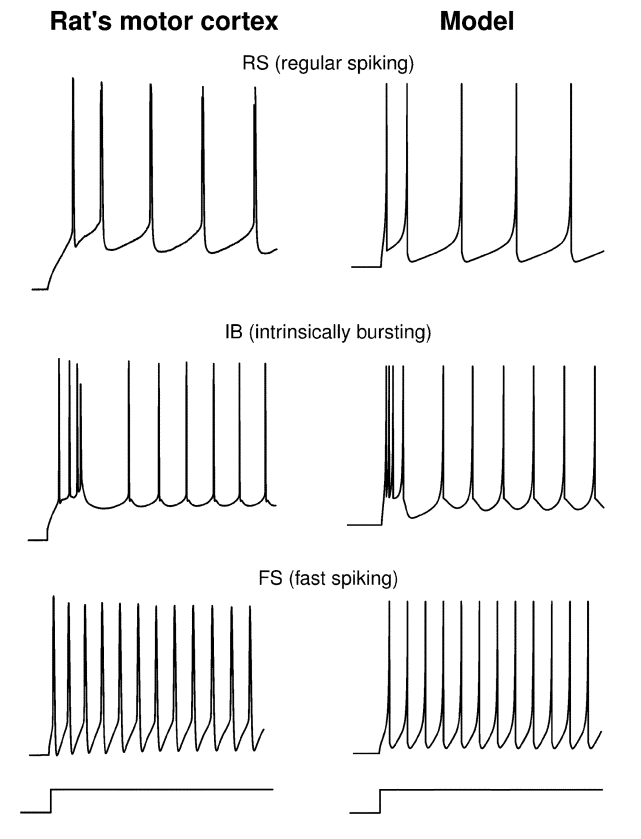
\includegraphics[height=4.3cm]{patrones_disparo_izhikevich.png}
    \end{column}
  \end{columns}
  \vspace{-2pt}
  \begin{alertblock}{¿Por qué Izhikevich?}
    \footnotesize Riqueza dinámica cercana a modelos tipo Hodgkin-Huxley, a un costo computacional cercano al de integrate-and-fire: permite evaluar miles de configuraciones de red dentro del ciclo evolutivo.
  \end{alertblock}
\end{frame}

% ---------------------------------------------------------------------
\begin{frame}{Codificación y decodificación de espigas}
  \begin{center}
  \begin{tikzpicture}[scale=0.82, every node/.style={transform shape}, font=\small]
    % Valor normalizado
    \node[draw,rounded corners,fill=usachred!10,minimum height=1cm] (val) at (0,0) {$x_i \in [0,1]$};

    % Poisson
    \node[draw,rounded corners,fill=lightbg,minimum height=1cm,align=center] (poi) at (3.3,1.3) {Poisson\\[-1pt]\scriptsize (rate coding)};
    \draw[-{Latex}] (val) -- (poi);
    \draw[thick] (2.1,0.55) -- (4.5,0.55);
    \foreach \x in {2.35,2.55,2.95,3.15,3.55,3.85,4.1,4.3} \draw[semgreen,line width=1pt] (\x,0.4) -- (\x,0.7);

    % TTFS
    \node[draw,rounded corners,fill=lightbg,minimum height=1cm,align=center] (ttfs) at (3.3,-1.3) {TTFS\\[-1pt]\scriptsize (latencia)};
    \draw[-{Latex}] (val) -- (ttfs);
    \draw[thick] (2.1,-1.95) -- (4.5,-1.95);
    \draw[usachred,line width=1.4pt] (2.6,-2.1) -- (2.6,-1.8);
    \node[below,font=\scriptsize] at (2.6,-2.15) {1$^{\text{er}}$ spike};

    % Red
    \node[draw,rounded corners,fill=usachred!10,minimum height=2.3cm,minimum width=1.6cm,align=center] (red) at (6.2,0) {Red\\SNN\\(Izhikevich)};
    \draw[-{Latex}] (4.5,0.55) .. controls (5.3,0.55) .. (red.north west);
    \draw[-{Latex}] (4.5,-1.95) .. controls (5.3,-1.95) .. (red.south west);

    % Conteo de salida
    \node[align=center] (cnt) at (9,0.9) {\scriptsize conteo espigas};
    \draw[-{Latex}] (red) -- (7.9,0);
    \draw[fill=semgreen!70] (7.9,-0.9) rectangle (8.3,1.1);
    \draw[fill=usachred!60] (8.5,-0.9) rectangle (8.9,-0.1);
    \node[below,font=\scriptsize] at (8.1,-0.9) {c0};
    \node[below,font=\scriptsize] at (8.7,-0.9) {c1};

    % Argmax
    \node[draw,rounded corners,fill=usachred,text=white,align=center] (arg) at (11,0) {\scriptsize\textbf{Rate}\\[-2pt]\scriptsize\textbf{argmax}};
    \draw[-{Latex}] (8.9,0) -- (arg);
    \draw[-{Latex}] (arg) -- ++(1.6,0) node[right,align=left,font=\scriptsize] {clase\\predicha};
  \end{tikzpicture}
  \end{center}
  \begin{itemize}\small
    \item \textbf{Poisson}: espiga por paso con probabilidad $\propto$ valor normalizado (tasa media).
    \item \textbf{TTFS}: a lo sumo una espiga; la latencia codifica la intensidad (más alto $\Rightarrow$ más temprano).
    \item \textbf{Rate argmax}: cuenta espigas de salida en la ventana y elige la neurona con más conteo (empates $\rightarrow$ azar uniforme).
  \end{itemize}
  \centering\footnotesize\textit{Este esquema explica más adelante las diferencias de tiempo de cómputo entre algoritmos.}
\end{frame}

% ---------------------------------------------------------------------
\begin{frame}{Multiobjetivo, esparsidad e hipervolumen}
  \begin{columns}[T]
    \begin{column}{0.5\textwidth}
      \small
      \begin{itemize}
        \item $x \succ y$ (\textbf{dominancia}): $x$ no es peor que $y$ en ningún objetivo y es mejor en al menos uno.
        \item \textbf{Frente de Pareto}: soluciones no dominadas $\Rightarrow$ mejores compromisos posibles.
        \item \textbf{Hipervolumen (HV)}: volumen del espacio objetivo dominado respecto a un punto de referencia $r$.
      \end{itemize}
      \[
        HV(A,r)=\Lambda\!\Big(\bigcup_{a\in A}[f_1(a),r_1]\times[f_2(a),r_2]\Big)
      \]
      \begin{alertblock}{¿Por qué importa?}
        \footnotesize Integra convergencia \emph{y} diversidad en un solo escalar, compatible con dominancia de Pareto. En este trabajo $r=(1,1)$, fijo para todo algoritmo/dataset.
      \end{alertblock}
    \end{column}
    \begin{column}{0.5\textwidth}
      \centering
      \begin{tikzpicture}[scale=3.1, font=\scriptsize]
        \draw[-{Latex}] (0,0) -- (1.15,0) node[right] {$f_1$ (complejidad)};
        \draw[-{Latex}] (0,0) -- (0,1.15) node[above] {$f_2$ (error)};
        % puntos del frente (orden por f1 ascendente, f2 descendente)
        \def\pts{(0.08,0.85),(0.18,0.55),(0.32,0.38),(0.5,0.27),(0.72,0.18)}
        % sombreado HV: rectangulos desde cada punto hasta r=(1,1)
        \foreach \p in \pts {
          \fill[semgreen!45] \p rectangle (1,1);
        }
        \draw[usachred,thick] plot coordinates {(0.08,0.85)(0.18,0.55)(0.32,0.38)(0.5,0.27)(0.72,0.18)};
        \foreach \p in \pts { \fill[usachred] \p circle (0.012); }
        \draw[fill=black] (1,1) circle (0.014) node[below left,font=\tiny] {$r=(1,1)$};
      \end{tikzpicture}
      \small\textit{Área verde = HV(A,r)}
    \end{column}
  \end{columns}
\end{frame}

% =====================================================================
\section{Metodología}
% =====================================================================
\begin{frame}{Formulación del problema Sparse SNN}
  \begin{columns}[T]
    \begin{column}{0.48\textwidth}
      \small
      \[
        f_1(x)=\frac{\|x\|_0}{\|x\|} \qquad f_2(x)=1-\mathrm{Acc}(x)
      \]
      \begin{itemize}
        \item $x=(w_0,\ldots,w_{D-1})\in[0,1]^D$: vector real; $w_i=0$ desactiva la sinapsis.
        \item Dimensión del espacio de decisión:
      \end{itemize}
      \[
        D=(n_F+1)\cdot n_H + n_H\cdot n_O
      \]
      \small La topología es fija; el \emph{genotipo} decide simultáneamente presencia de conexión e intensidad.
    \end{column}
    \begin{column}{0.52\textwidth}
      \centering
      \begin{tikzpicture}[scale=0.62, every node/.style={transform shape},
          x=1.5cm, y=0.8cm,
          neuron/.style={circle, draw, minimum size=0.65cm},
          bias/.style={circle, draw, dashed, minimum size=0.65cm},
          conn/.style={-, gray, opacity=0.5}]
        \foreach \i/\y in {1/2, 2/1, 3/0, 4/-1, 5/-2}
            \node[neuron] (I\i) at (0,\y) {};
        \node[bias] (B) at (0,-3) {$1$};
        \foreach \i/\y in {1/2.5, 2/1.5, 3/0.5, 4/-0.5, 5/-1.5, 6/-2.5}
            \node[neuron] (H\i) at (3,\y) {};
        \node[neuron] (O1) at (6,0.75) {};
        \node[neuron] (O2) at (6,-0.75) {};
        \foreach \i in {1,...,5}
            \foreach \j in {1,...,6}
                \draw[conn] (I\i) -- (H\j);
        \foreach \j in {1,...,6}
            \draw[conn] (B) -- (H\j);
        \foreach \j in {1,...,6}{
            \draw[conn] (H\j) -- (O1);
            \draw[conn] (H\j) -- (O2);
        }
        \node[align=center] at (0,-4.1) {\small Entrada\\($n_F$+bias)};
        \node[align=center] at (3,-4.1) {\small Oculta ($n_H$)};
        \node[align=center] at (6,-4.1) {\small Salida (2 clases)};
      \end{tikzpicture}
      \small\textit{Figura 4.1 --- topología \textit{feedforward} del problema Sparse SNN}
    \end{column}
  \end{columns}
\end{frame}

% ---------------------------------------------------------------------
\begin{frame}{Los dos algoritmos: S-NSGA-II y MOEA-CKF}
  \begin{columns}[T]
    \begin{column}{0.46\textwidth}
      \small
      \textbf{Selección:} Taxonomía de SMOEAs $\to$ preselección por familia $\to$ selección final con criterios:
      \begin{itemize}
        \item Código disponible en PlatEMO
        \item Datasets reportados en el estudio original
        \item Resuelve tareas de \textit{NN training}
      \end{itemize}
      \vspace{4pt}
      \textbf{S-NSGA-II}: vector único, operadores \texttt{S-SBX}/\texttt{S-PM} actúan directamente sobre $x$.\\[4pt]
      \textbf{MOEA-CKF}: codificación \textbf{bi-nivel}, $x_j = m_j \cdot d_j$.
    \end{column}
    \begin{column}{0.54\textwidth}
      \centering
      \begin{tikzpicture}[scale=0.72, every node/.style={transform shape}, font=\scriptsize]
        \node[anchor=west] at (-1.1,2.1) {\textbf{S-NSGA-II}};
        \foreach \i/\v in {0/0.6,1/0,2/0.9,3/0,4/0,5/0.3,6/0.7,7/0} {
          \pgfmathsetmacro{\c}{100-\v*100}
          \ifdim \v pt=0pt
            \draw[fill=white] (\i*0.62,1.5) rectangle ++(0.55,0.55);
            \node at (\i*0.62+0.28,1.78) {0};
          \else
            \draw[fill=usachred!\c!usachred] (\i*0.62,1.5) rectangle ++(0.55,0.55);
          \fi
        }
        \node[anchor=west,font=\tiny] at (-1.1,1.25) {$x$: vector real único};

        \node[anchor=west] at (-1.1,0.1) {\textbf{MOEA-CKF}};
        \foreach \i/\m in {0/1,1/0,2/1,3/0,4/0,5/1,6/1,7/0} {
          \ifnum\m=1
            \draw[fill=black!75] (\i*0.62,-0.5) rectangle ++(0.55,0.4);
            \node[white] at (\i*0.62+0.28,-0.3) {1};
          \else
            \draw[fill=white] (\i*0.62,-0.5) rectangle ++(0.55,0.4);
            \node at (\i*0.62+0.28,-0.3) {0};
          \fi
        }
        \node[anchor=west,font=\tiny] at (-1.1,-0.3) {$m$};
        \node at (2.2,-0.9) {$\times$};
        \foreach \i/\v in {0/0.7,1/0.4,2/0.9,3/0.2,4/0.5,5/0.3,6/0.8,7/0.1} {
          \pgfmathsetmacro{\c}{100-\v*100}
          \draw[fill=usachred!\c!usachred] (\i*0.62,-1.5) rectangle ++(0.55,0.4);
        }
        \node[anchor=west,font=\tiny] at (-1.1,-1.3) {$d$};
        \node at (2.2,-1.9) {$=$};
        \foreach \i/\v/\m in {0/0.7/1,1/0.4/0,2/0.9/1,3/0.2/0,4/0.5/0,5/0.3/1,6/0.8/1,7/0.1/0} {
          \ifnum\m=1
            \pgfmathsetmacro{\c}{100-\v*100}
            \draw[fill=usachred!\c!usachred] (\i*0.62,-2.5) rectangle ++(0.55,0.4);
          \else
            \draw[fill=white] (\i*0.62,-2.5) rectangle ++(0.55,0.4);
            \node[font=\tiny] at (\i*0.62+0.28,-2.3) {0};
          \fi
        }
        \node[anchor=west,font=\tiny] at (-1.1,-2.3) {$x=m\cdot d$};
      \end{tikzpicture}
    \end{column}
  \end{columns}
  \vspace{2pt}
  \centering\footnotesize\textit{Esta diferencia explica, más adelante, el patrón de conectividad de cada algoritmo.}
\end{frame}

% ---------------------------------------------------------------------
\begin{frame}{Datasets y diseño experimental}
  \begin{table}
  \centering\small
  \begin{tabular}{clcccc}
    \toprule
    N\textdegree & Dataset & Usado en & Muestras & Características & Clases \\
    \midrule
    1 & Statlog Australian & S-NSGA-II & 690  & 14 & 2 \\
    2 & Climate            & S-NSGA-II & 540  & 18 & 2 \\
    3 & Statlog German     & S-NSGA-II & 1000 & 24 & 2 \\
    4 & Connectionist Bench Sonar & MOEA-CKF & 208 & 60 & 2 \\
    \bottomrule
  \end{tabular}
  \end{table}
  \small
  \textbf{Tres conjuntos experimentales:}
  \begin{itemize}
    \item \textbf{Referencia}: comparación principal SNN vs.\ SNN + tiempo de cómputo.
    \item \textbf{Remuestreo}: ¿el \textit{bootstrap} de $f_2$ mejora o empeora el HV?
    \item \textbf{ANN}: SNN (C++) vs.\ ANN original de PlatEMO/MATLAB.
  \end{itemize}
  \begin{alertblock}{Rigor experimental}
    \footnotesize \textbf{31 corridas pareadas por semilla} por combinación algoritmo-dataset; \texttt{maxFE} igualado entre algoritmos en cada dataset.
  \end{alertblock}
\end{frame}

% ---------------------------------------------------------------------
\begin{frame}{Rigor estadístico}
  \begin{columns}[T]
    \begin{column}{0.46\textwidth}
      \small
      \begin{itemize}
        \item \textbf{Wilcoxon signed-rank} (pareado por semilla): SNN vs.\ SNN, remuestreo, tiempo.
        \item \textbf{Mann-Whitney U} (no pareado): SNN vs.\ ANN (semillas/RNG no equivalentes).
        \item \textbf{\Atwelve\ de Vargha-Delaney}: tamaño de efecto, umbrales est\'andar (insignificante/pequeño/mediano/grande).
        \item \textbf{Holm-Bonferroni}: corrección por comparaciones múltiples, por familia de tests.
      \end{itemize}
    \end{column}
    \begin{column}{0.54\textwidth}
      \centering
      \begin{tikzpicture}[scale=0.85, every node/.style={transform shape}, font=\small]
        \node[draw,rounded corners,minimum width=6.6cm,minimum height=3.6cm,fill=usachred!8] (outer) at (0,0) {};
        \node[anchor=north,font=\bfseries\small] at (outer.north) [yshift=-4pt] {Optuna / TPE (bucle externo)};
        \node[draw,rounded corners,minimum width=4.8cm,minimum height=2.3cm,fill=usachred!18] (mid) at (0,-0.4) {};
        \node[anchor=north,font=\bfseries\small] at (mid.north) [yshift=-4pt] {SMOEA (S-NSGA-II / MOEA-CKF)};
        \node[draw,rounded corners,minimum width=2.8cm,minimum height=1cm,fill=usachred!45,text=white] (inner) at (0,-0.9) {\small Simulador SNN};
        \draw[-{Latex},semgreen,thick] (inner.east) .. controls +(1.3,0.3) and +(0.2,-0.9) .. (mid.east) node[midway,right,font=\tiny,text=black] {$f_1,f_2$};
        \draw[-{Latex},usachred,thick] (mid.east) .. controls +(1.9,0.6) and +(0.2,-1.1) .. (outer.east) node[midway,right,font=\tiny,text=black,xshift=2pt] {frente final};
        \node[below=0.15cm of outer,font=\tiny] {objetivo externo: HV medio $\leftarrow$ frente final $\leftarrow$ $(f_1,f_2)$};
      \end{tikzpicture}
    \end{column}
  \end{columns}
\end{frame}

% =====================================================================
\section{Implementación}
% =====================================================================
\begin{frame}{Arquitectura y validación}
  \begin{columns}[T]
    \begin{column}{0.55\textwidth}
      \small \textbf{Cinco módulos:}
      \begin{enumerate}\small
        \item Módulo evolutivo (Problema/Solución, operadores)
        \item Simulador SNN (Izhikevich, codificación/decodificación)
        \item Manejo de datasets
        \item Métricas (objetivos, HV)
        \item Configuración experimental (orquestación)
      \end{enumerate}
    \end{column}
    \begin{column}{0.45\textwidth}
      \centering
      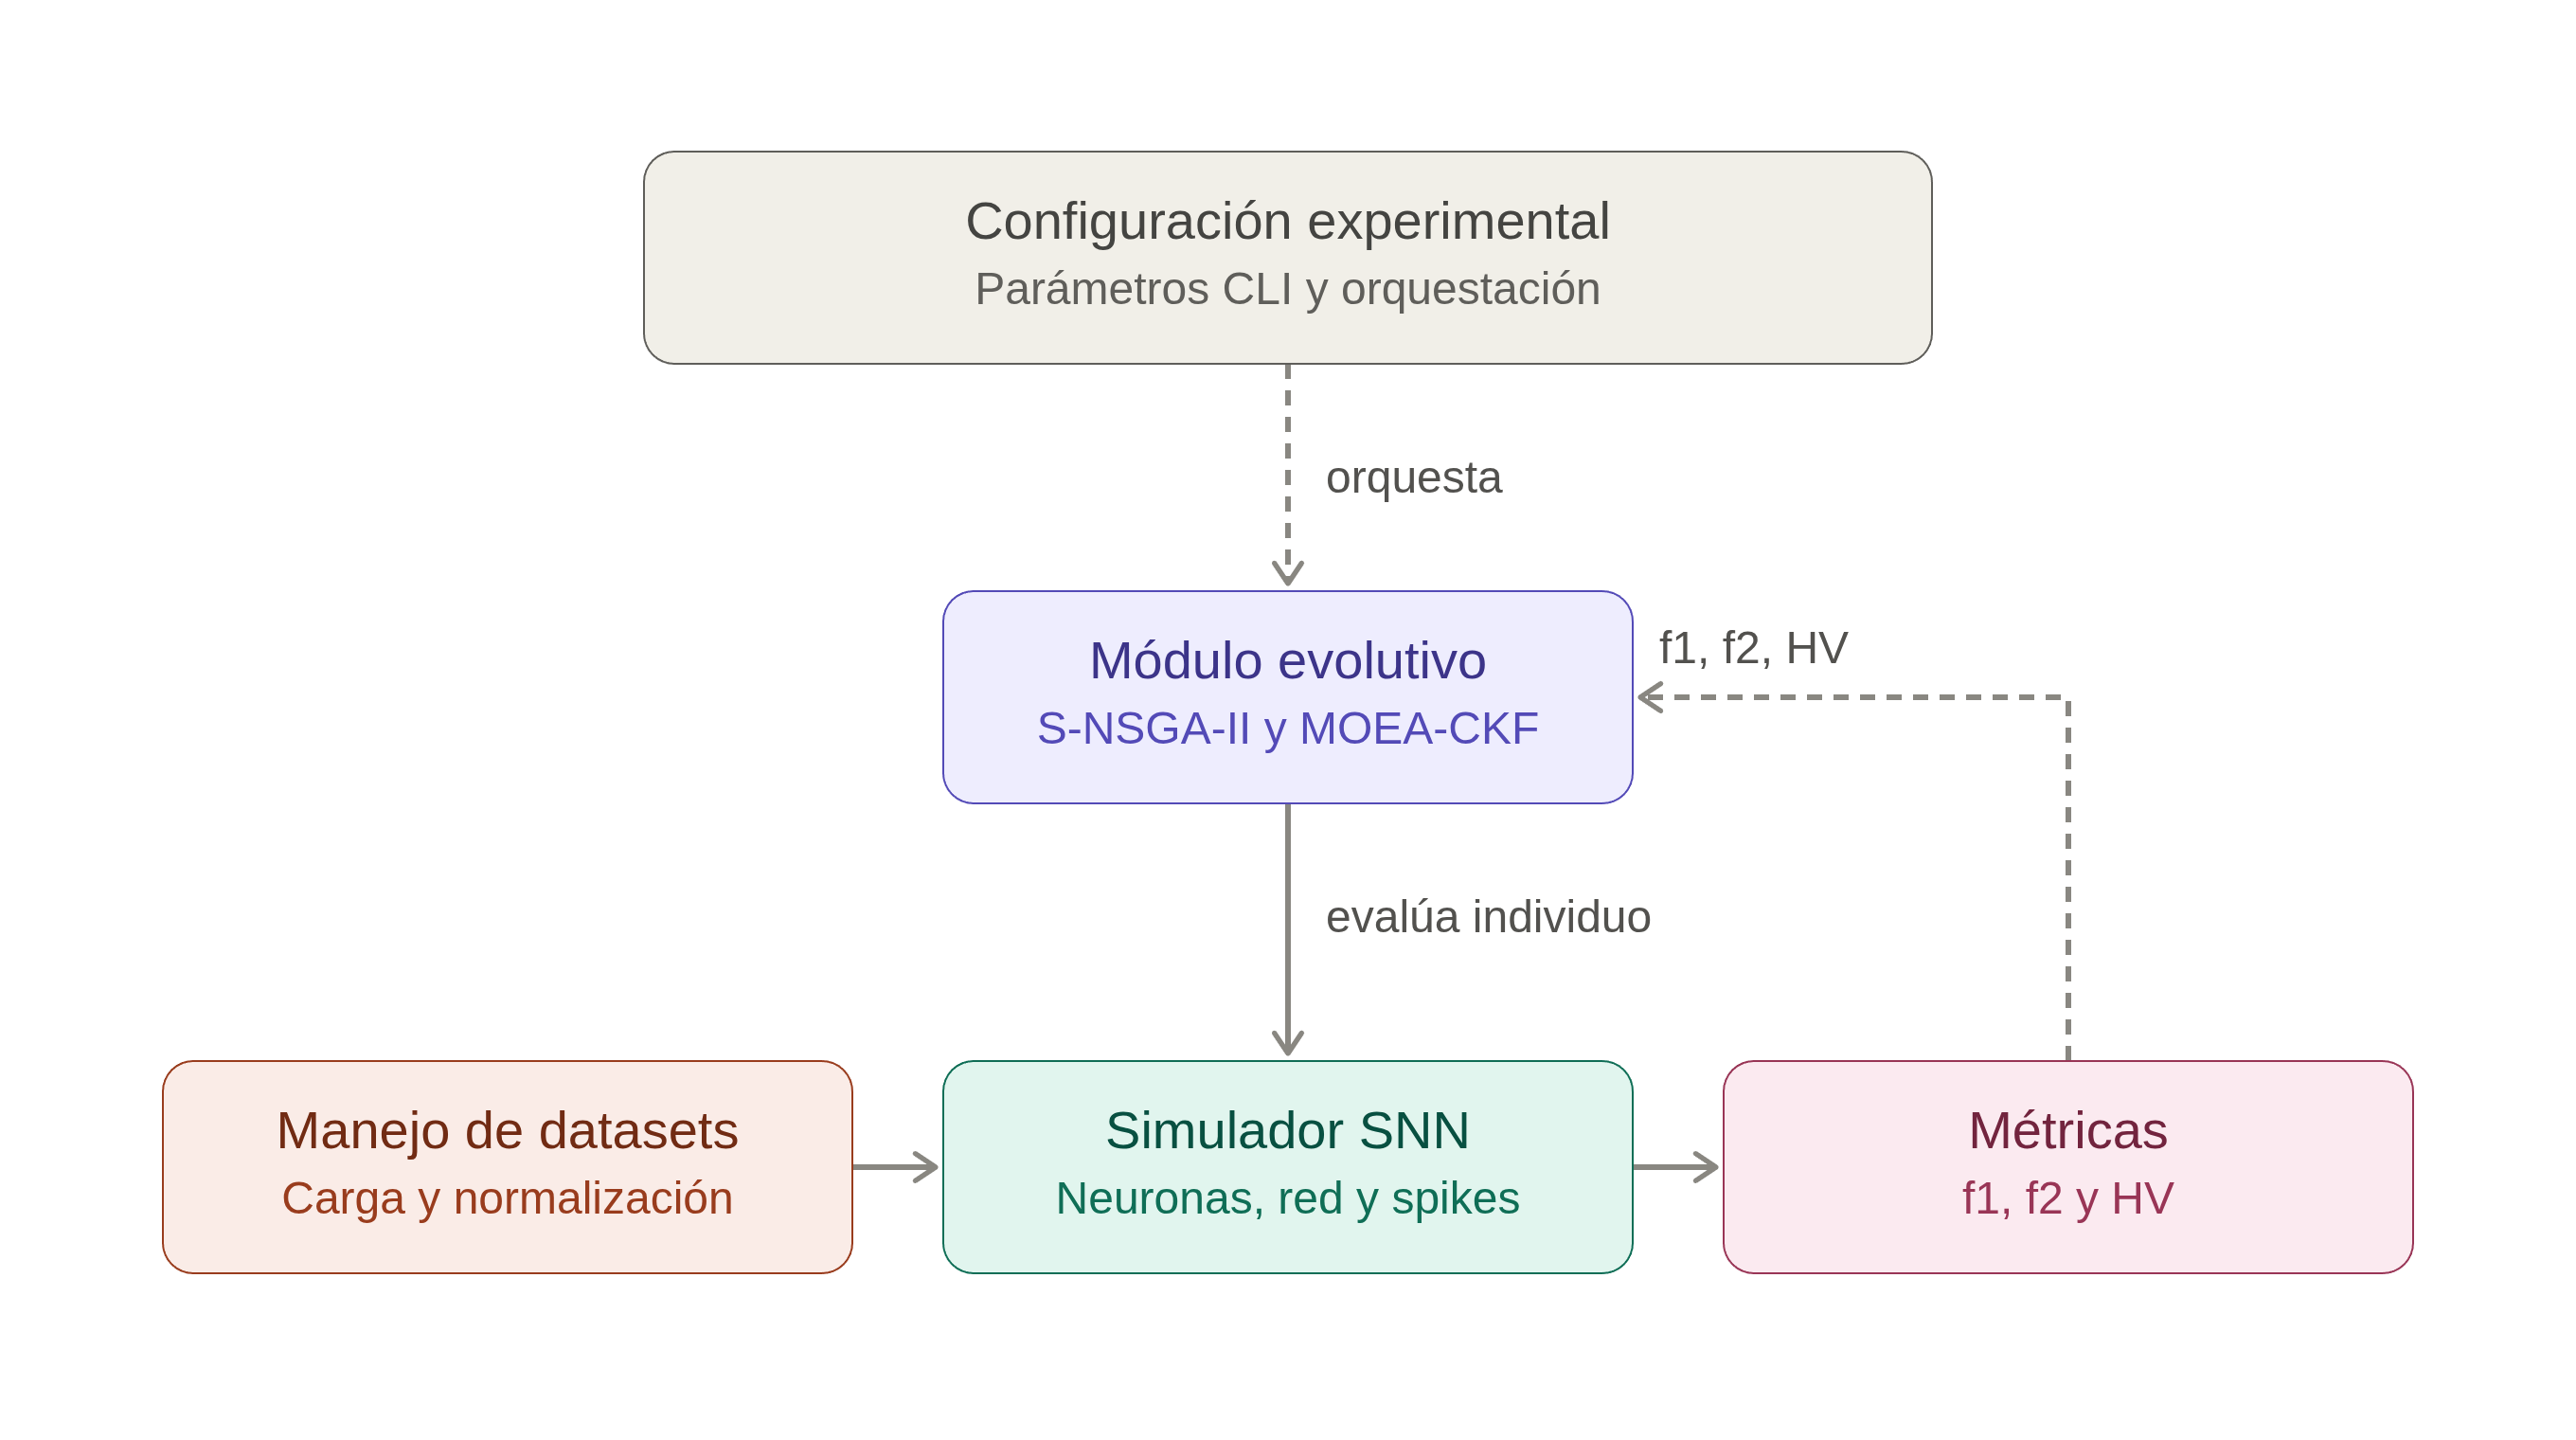
\includegraphics[width=0.95\linewidth]{modulos_sistema_snn.png}
    \end{column}
  \end{columns}
  \begin{alertblock}{Migración PlatEMO/MATLAB $\to$ C++}
    \footnotesize Equivalencia \textbf{funcional por construcción} (misma definición matemática/orden lexicográfico), \emph{no} numérica: los RNG difieren entre MATLAB y C++. Limitación reconocida explícitamente.
  \end{alertblock}
  \begin{block}{Validación}
    \footnotesize \textbf{33 pruebas unitarias} (Catch2/CTest): neurona (3), red (7), simulador (9), codificación (9), decodificación (5).
  \end{block}
\end{frame}

% =====================================================================
\section{Resultados}
% =====================================================================
\begin{frame}{Selección del simulador SNN}
  \begin{columns}[T]
    \begin{column}{0.5\textwidth}
      \small
      \begin{itemize}
        \item \textbf{18/18} comparaciones por pares: $U=0$, $p\approx3\times10^{-11}$.
        \item De \textbf{900} comparaciones posibles (30$\times$30), \textit{snn-simulator} fue menor en las 900 --- separación total.
        \item Construcción de red en \textbf{microsegundos}: 3--4 órdenes de magnitud bajo NEST y ANNarchy.
      \end{itemize}
      \begin{alertblock}{Honestidad}
        \footnotesize Desventaja: $\approx$9\,MB de memoria adicional frente a ANNarchy --- irrelevante frente a la ventaja temporal.
      \end{alertblock}
    \end{column}
    \begin{column}{0.5\textwidth}
      \centering
      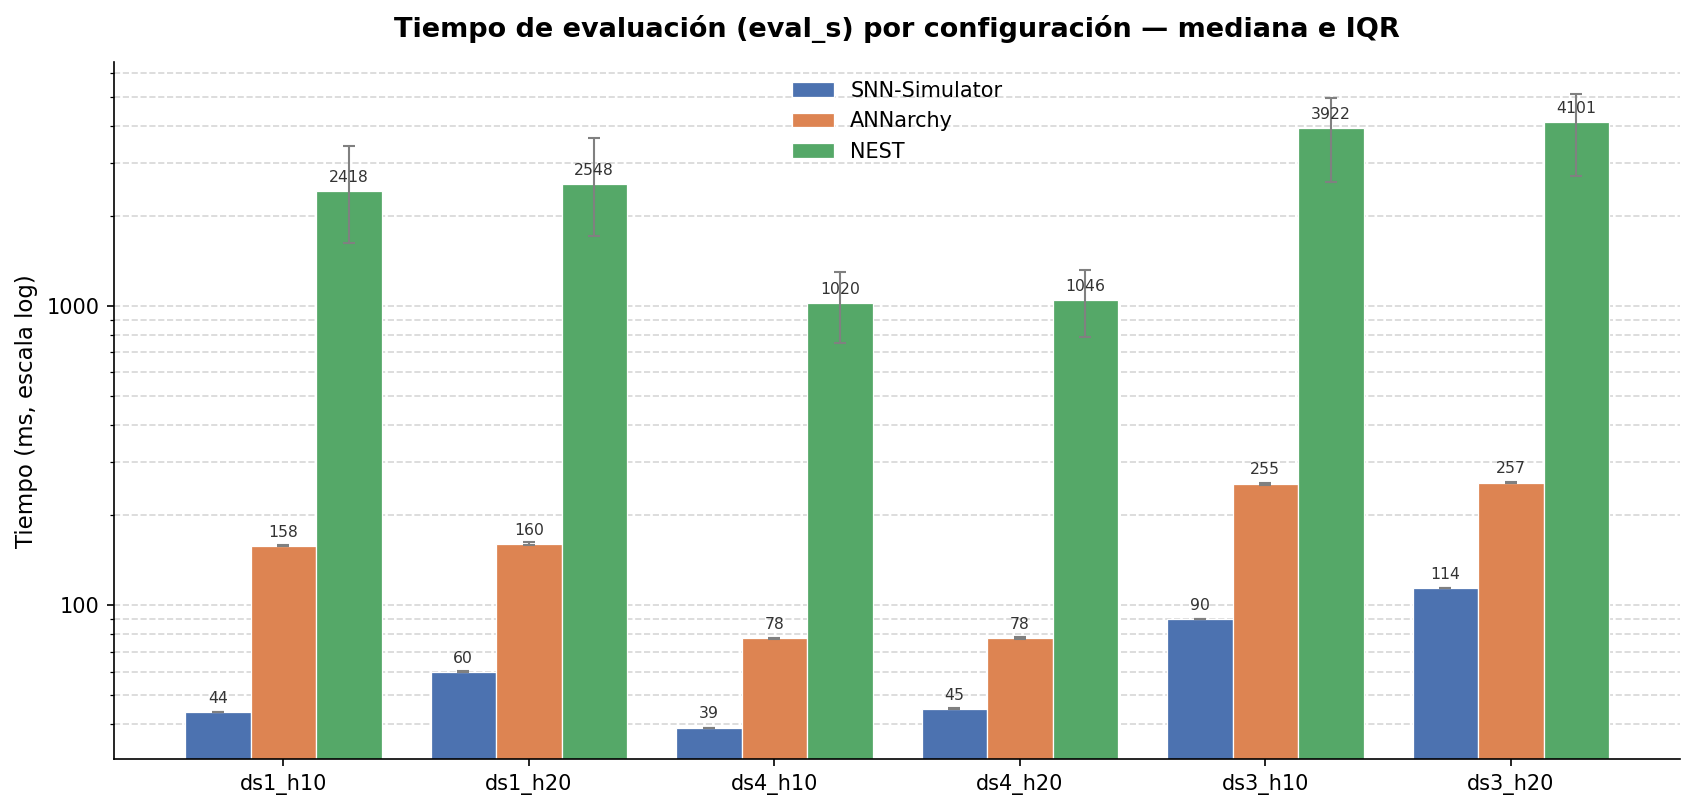
\includegraphics[width=\linewidth]{plot_eval_s_median_iqr.png}\\
      \footnotesize Figura 6.1 --- tiempo de evaluación por configuración
    \end{column}
  \end{columns}
\end{frame}

% ---------------------------------------------------------------------
\begin{frame}{Hiperparámetros: qué domina}
  \begin{columns}[T]
    \begin{column}{0.42\textwidth}
      \small
      \begin{itemize}
        \item Ocho estudios independientes (algoritmo $\times$ dataset).
        \item \textbf{\texttt{wScale}} concentra la mayor parte de la varianza explicada del HV en \textbf{6 de 8} estudios.
        \item Ejemplo \texttt{ds2}: 95.9\% (MOEA-CKF), 96.2\% (S-NSGA-II).
        \item Excepción: \texttt{ds4} (60 características) --- \texttt{architecture} domina en MOEA-CKF (52.7\%); reparto \texttt{wScale}/\texttt{sGap} en S-NSGA-II.
      \end{itemize}
    \end{column}
    \begin{column}{0.58\textwidth}
      \centering
      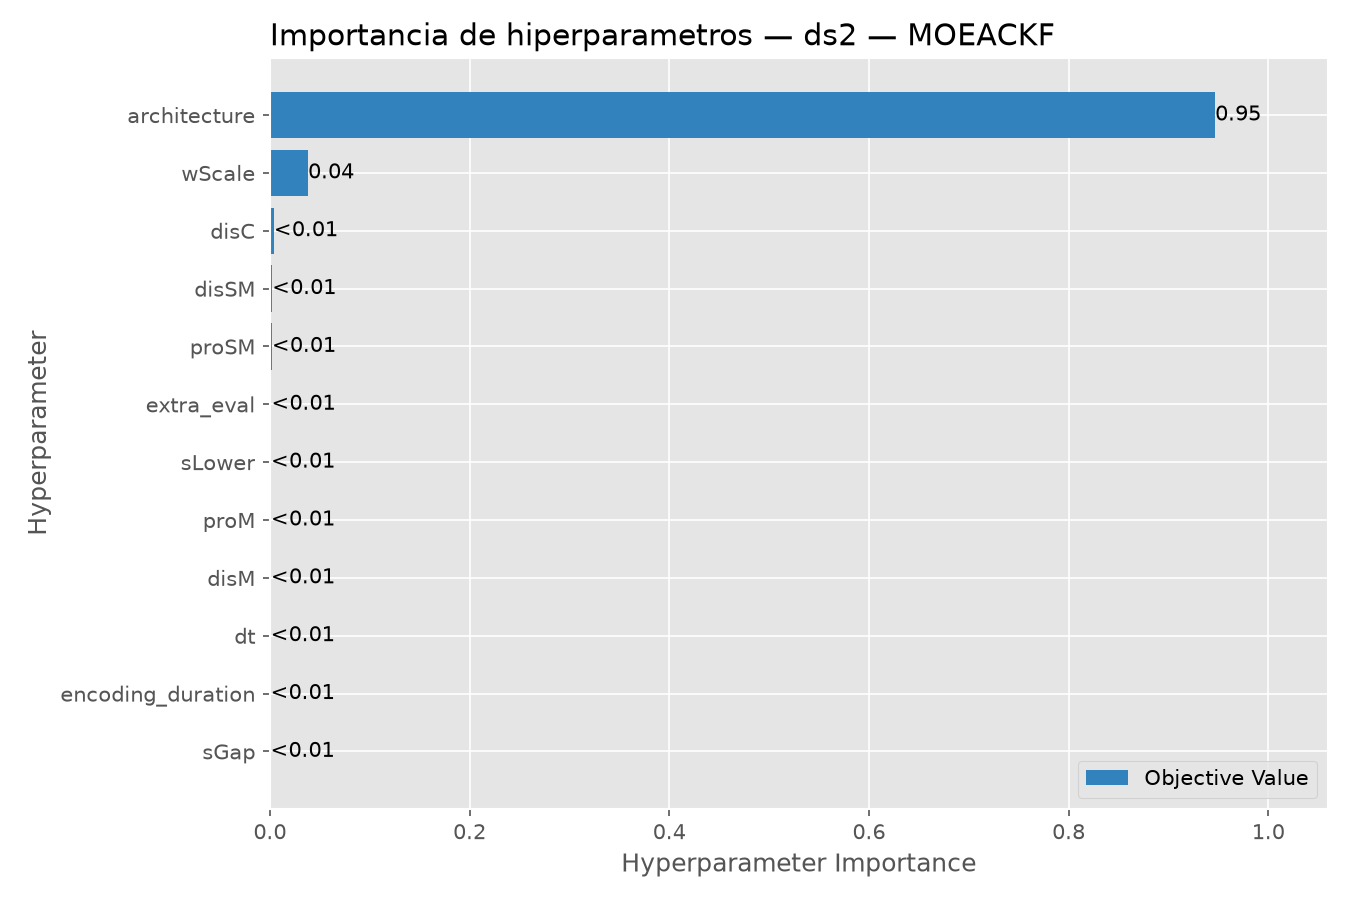
\includegraphics[width=0.49\linewidth]{importancia_MOEACKF_ds2.png}%
      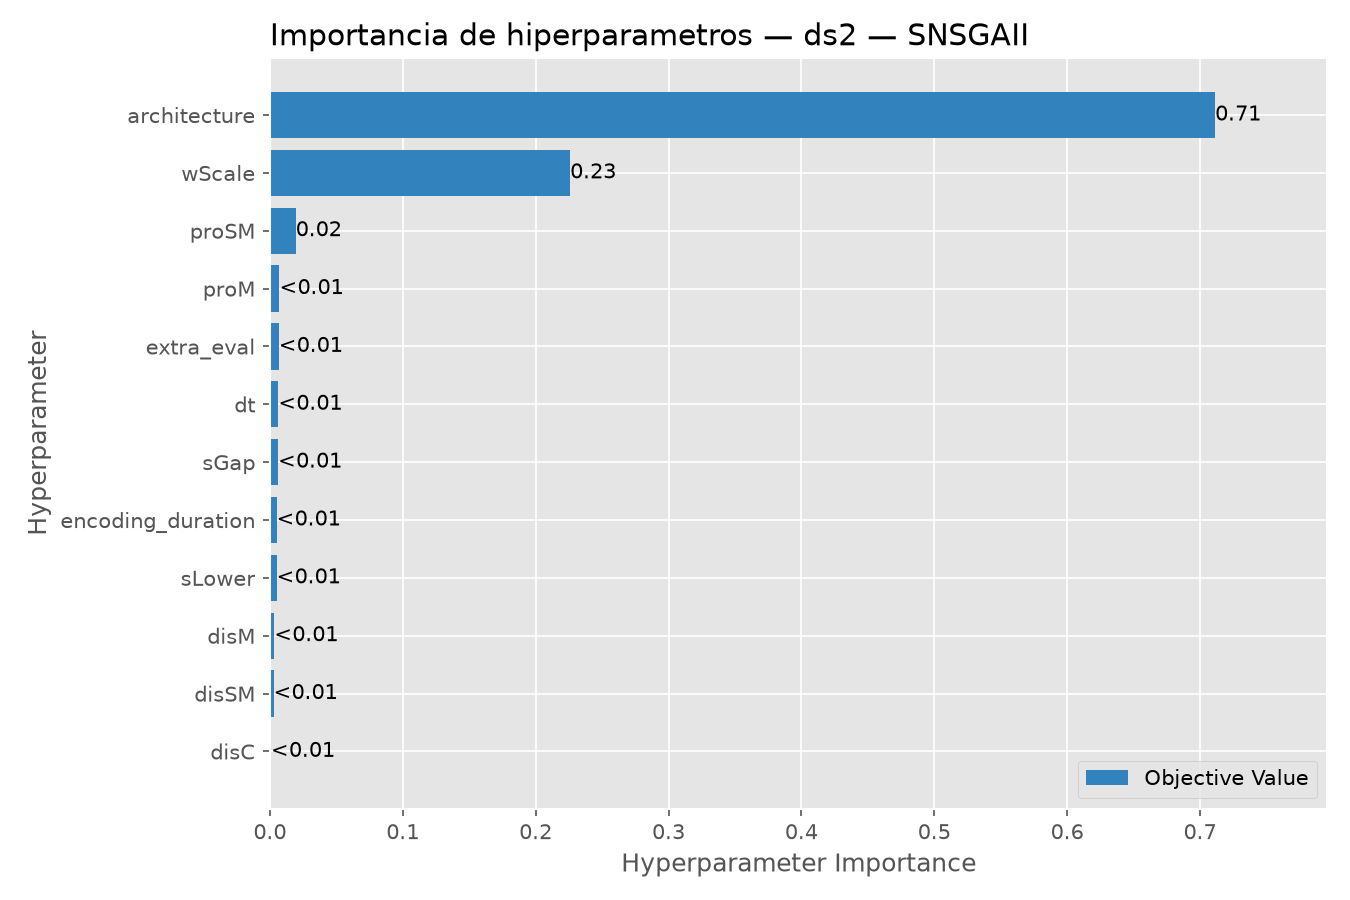
\includegraphics[width=0.49\linewidth]{importancia_SNSGAII_ds2.png}\\[2pt]
      \footnotesize \texttt{ds2}: caso representativo (izq.\ MOEA-CKF, der.\ S-NSGA-II; resto en \textit{backup})
    \end{column}
  \end{columns}
\end{frame}

% ---------------------------------------------------------------------
\begin{frame}{Hipervolumen: MOEA-CKF vs.\ S-NSGA-II}
  \begin{table}
  \centering\scriptsize
  \begin{tabular}{cllccc}
    \toprule
    \textbf{Dataset} & \textbf{MOEA-CKF} & \textbf{S-NSGA-II} & \textbf{$p$ Wilcoxon} & \textbf{$p$ corr.} & \Atwelve \\
    \midrule
    1 & \cellcolor{semgreen!25}$0.8705\,[0.8704,0.8721]$ & $0.8459\,[0.7895,0.8712]$ & $1.18\times10^{-4}$* & $4.74\times10^{-4}$* & 0.710 \\
    2 & \cellcolor{semgreen!25}$0.9298\,[0.9277,0.9319]$ & $0.9278\,[0.9277,0.9278]$ & $0.0289$*  & $0.0408$*  & 0.645 \\
    3 & $0.7563\,[0.7484,0.7634]$ & $0.7520\,[0.7498,0.7566]$ & $0.2023$   & $0.2075$   & 0.645 \\
    4 & $0.8043\,[0.7936,0.8283]$ & \cellcolor{semgreen!25}$0.8229\,[0.8020,0.8418]$ & $0.0051$*  & $0.0254$*  & 0.290 \\
    \bottomrule
  \end{tabular}
  \end{table}
  \small
  \begin{itemize}
    \item Rendimiento \textbf{estadísticamente equivalente} en agregado.
    \item \textbf{MOEA-CKF} mejor en \texttt{ds1}--\texttt{ds2}; \textbf{sin diferencia} en \texttt{ds3}; \textbf{S-NSGA-II} mejor en \texttt{ds4} (mayor dimensionalidad, 60 características).
  \end{itemize}
\end{frame}

% ---------------------------------------------------------------------
\begin{frame}{Frentes de Pareto y bandas de complejidad}
  \begin{columns}[T]
    \begin{column}{0.5\textwidth}
      \centering
      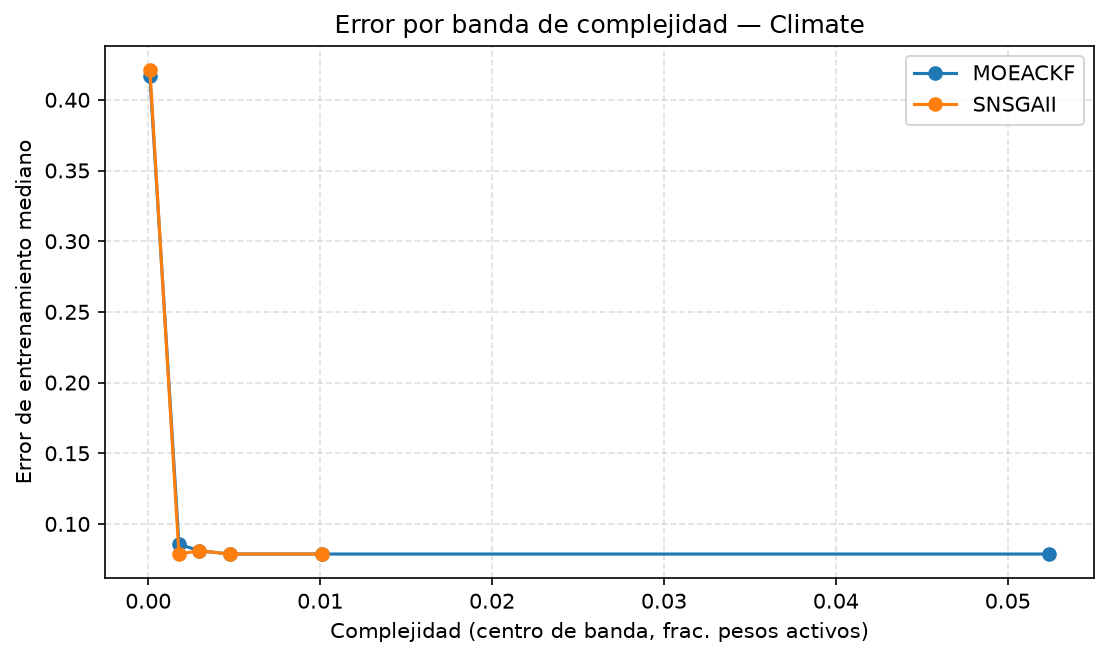
\includegraphics[height=3.5cm]{ds2_complexity_bands.png}\\
      \scriptsize \texttt{ds2}: S-NSGA-II encuentra redes mucho más esparsas (\Atwelve=0.919) con error casi igual.
    \end{column}
    \begin{column}{0.5\textwidth}
      \centering
      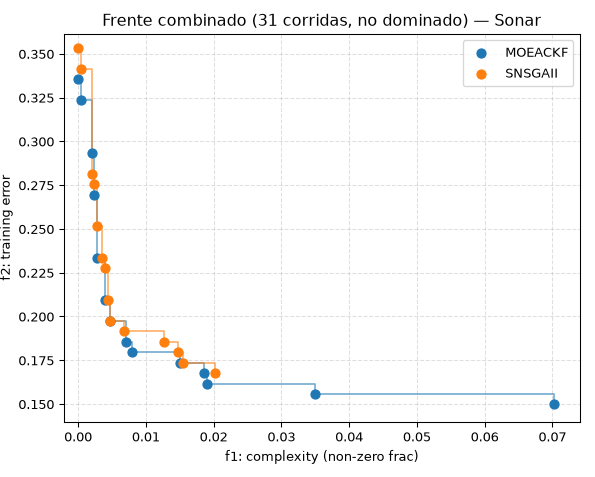
\includegraphics[height=3.5cm]{ds4_combined_front.png}\\
      \scriptsize \texttt{ds4}: 84.6\% del frente de MOEA-CKF dominado --- el resultado más asimétrico.
    \end{column}
  \end{columns}
  \begin{alertblock}{Dos métricas, dos mensajes}
    \scriptsize El HV agregado y la dominancia punto a punto (C-metric) miden aspectos \emph{distintos} del frente: solo coinciden claramente en \texttt{ds4}.
  \end{alertblock}
\end{frame}

% ---------------------------------------------------------------------
\begin{frame}{Tiempo de cómputo}
  \begin{table}
  \centering\scriptsize
  \begin{tabular}{ccccc}
    \toprule
    \textbf{Dataset} & \textbf{MOEA-CKF} & \textbf{S-NSGA-II} & \textbf{$p$ (Wilcoxon)} & \Atwelve \\
    \midrule
    1 & $275.4\,[259.7,284.3]$ s & \cellcolor{semgreen!25}$159.5\,[155.3,165.3]$ s & $9.31\times10^{-10}$* & 1.000 \\
    2 & \cellcolor{semgreen!25}$188.1\,[174.4,213.1]$ s & $223.4\,[204.0,243.8]$ s & $4.53\times10^{-4}$* & 0.226 \\
    3 & \cellcolor{semgreen!25}$627.8\,[578.8,664.6]$ s & $1026.0\,[995.4,1063.0]$ s & $9.31\times10^{-10}$* & 0.000 \\
    4 & $477.4\,[427.4,640.3]$ s & \cellcolor{semgreen!25}$167.4\,[166.5,170.9]$ s & $9.31\times10^{-10}$* & 1.000 \\
    \bottomrule
  \end{tabular}
  \end{table}
  \small
  \begin{itemize}
    \item El algoritmo \textbf{más rápido cambia según el codificador} que cada uno eligió en su propia búsqueda (Poisson vs.\ TTFS).
    \item \textbf{Excepción: \texttt{ds4}}, ambos usan TTFS y aun así S-NSGA-II gana con \Atwelve$=1.000$ $\Rightarrow$ aísla un \textbf{costo algorítmico propio} de MOEA-CKF.
  \end{itemize}
\end{frame}

% ---------------------------------------------------------------------
\begin{frame}{SNN vs.\ ANN}
  \small
  \begin{itemize}
    \item \textbf{El resultado más uniforme}: la ANN (PlatEMO/MATLAB) gana en HV y error en las \textbf{8/8} combinaciones evaluadas.
    \item \textbf{23 de 24} comparaciones (HV, error, complejidad) resultaron significativas tras corrección.
    \item Pero la \textbf{SNN es más esparsa}, marcadamente bajo S-NSGA-II (redes ANN casi densas en \texttt{ds2}/\texttt{ds3}, $\Atwelve=0.000$).
  \end{itemize}
  \vspace{-3pt}
  \begin{table}
  \centering\scriptsize
  \renewcommand{\arraystretch}{0.85}
  \begin{tabular}{lccc}
    \toprule
    \textbf{ds2, S-NSGA-II} & \textbf{SNN} & \textbf{ANN} & \Atwelve \\
    \midrule
    HV & $0.9278$ & $0.9477$ & 0.000 \\
    Complejidad & $0.0024$ & $0.9114$ & 0.000 \\
    Error & $0.0787$ & $0.0347$ & 1.000 \\
    \bottomrule
  \end{tabular}
  \end{table}
  \vspace{-3pt}
  \begin{alertblock}{Salvedad metodológica}
    \scriptsize La ANN \textbf{no} recibió ajuste bayesiano de hiperparámetros. No se oculta: es una limitación identificada, no un error.
  \end{alertblock}
\end{frame}

% ---------------------------------------------------------------------
\begin{frame}{Conectividad de las redes (I): el concepto}
  \begin{columns}[T]
    \begin{column}{0.55\textwidth}
      \small \textbf{Estados de una neurona oculta:}
      \begin{itemize}
        \item \textcolor{semgreen!70!black}{\textbf{Viva}}: entrada y salida activas (camino completo).
        \item \textcolor{semred}{\textbf{Muerta}}: sin ninguna conexión activa.
        \item \textcolor{orange!90!black}{\textbf{Sumidero}}: entrada activa, sin salida.
        \item \textcolor{yellow!70!orange}{\textbf{Fuente}}: salida activa, sin entrada.
      \end{itemize}
      \begin{alertblock}{Conexión inútil}
        \footnotesize Sinapsis activa que no puede formar parte de ningún camino completo entrada$\to$salida (llega a un sumidero o sale de una fuente).
      \end{alertblock}
    \end{column}
    \begin{column}{0.45\textwidth}
      \centering
      \begin{tikzpicture}[scale=0.85, every node/.style={transform shape},
          neuron/.style={circle,draw,minimum size=0.7cm}, font=\small]
        \node[neuron,fill=blue!15] (i1) at (0,1.2) {};
        \node[neuron,fill=blue!15] (i2) at (0,0) {};
        \node[neuron,fill=blue!15] (i3) at (0,-1.2) {};

        \node[neuron,fill=semgreen!60] (h1) at (2.4,1.5) {};
        \node[neuron,fill=semred!50] (h2) at (2.4,0.5) {};
        \node[neuron,fill=orange!60] (h3) at (2.4,-0.5) {};
        \node[neuron,fill=yellow!60] (h4) at (2.4,-1.5) {};

        \node[star,star points=5,draw,fill=red!70,minimum size=0.55cm] (o1) at (4.8,0.7) {};
        \node[star,star points=5,draw,fill=red!70,minimum size=0.55cm] (o2) at (4.8,-0.7) {};

        \draw[-{Latex},thick] (i1) -- (h1); \draw[-{Latex},thick] (i2) -- (h1);
        \draw[-{Latex},thick] (i1) -- (h3); \draw[-{Latex},thick,usachred,line width=1.1pt] (i3) -- (h3);
        \draw[-{Latex},thick] (h1) -- (o1);
        \draw[-{Latex},thick,usachred,line width=1.1pt] (h4) -- (o2);

        \node[below,font=\scriptsize] at (2.4,-2.1) {viva / muerta / sumidero / fuente};
        \draw[decorate,decoration={brace,amplitude=4pt}] (5.3,0.4) -- (5.3,-1.9) node[midway,right,font=\scriptsize,align=left,xshift=2pt] {sin conexión\\hacia esta clase};
      \end{tikzpicture}
      \footnotesize\centering Esquema mínimo (4 neuronas); conexiones inútiles resaltadas en rojo.
    \end{column}
  \end{columns}
\end{frame}

% ---------------------------------------------------------------------
\begin{frame}{Conectividad de las redes (II): resultados}
  \vspace{-2pt}
  \begin{table}
  \centering\small
  \renewcommand{\arraystretch}{0.85}
  \begin{tabular}{lrrrr}
    \toprule
    \textbf{Algoritmo} & \textbf{Corridas} & \textbf{Exactitud} (\%) & \textbf{\% salida desc.} & \textbf{\% conex.\ inútiles} \\
    \midrule
    MOEA-CKF  & 124 & 82.7 & \cellcolor{semgreen!25}21.0 & \cellcolor{semred!20}52.5 \\
    S-NSGA-II & 124 & 82.0 & \cellcolor{semred!20}51.6 & \cellcolor{semgreen!25}20.3 \\
    \bottomrule
  \end{tabular}
  \end{table}
  \vspace{-2pt}
  \small
  \begin{columns}[T]
    \begin{column}{0.5\textwidth}
      \footnotesize\textbf{Salidas desconectadas $\to$ desbalance de clases}: \texttt{ds2} clase minoritaria 8.5\%.
      \centering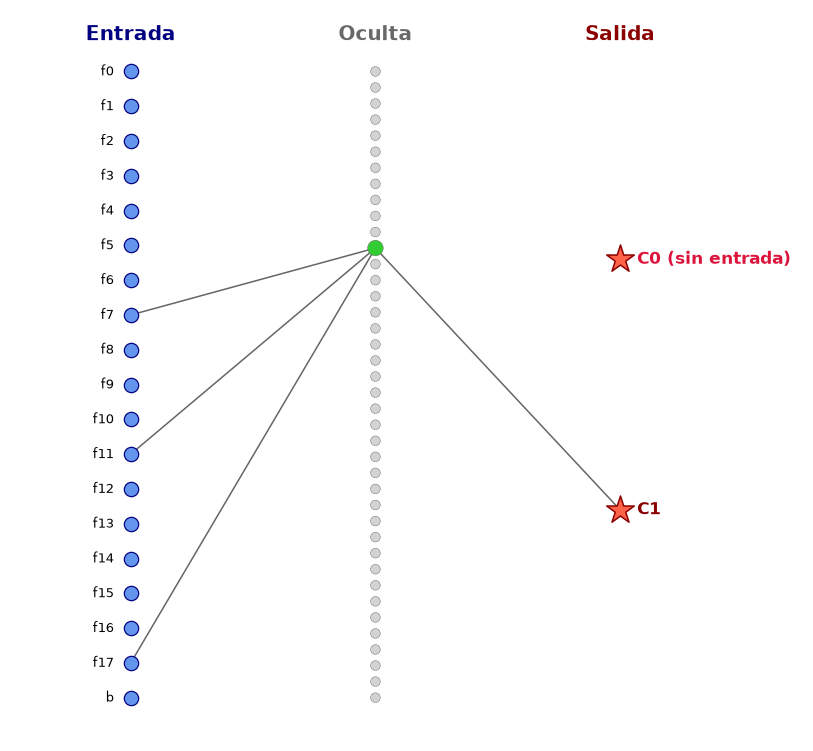
\includegraphics[height=3.1cm]{conectividad_ds2_snsgaii.png}
    \end{column}
    \begin{column}{0.5\textwidth}
      \footnotesize\textbf{Conexiones inútiles $\to$ asimetría estructural}: $n_F{+}1$ entradas vs.\ 2 salidas; 22.0\% (\texttt{ds1}) $\to$ 60.5\% (\texttt{ds4}).
      \centering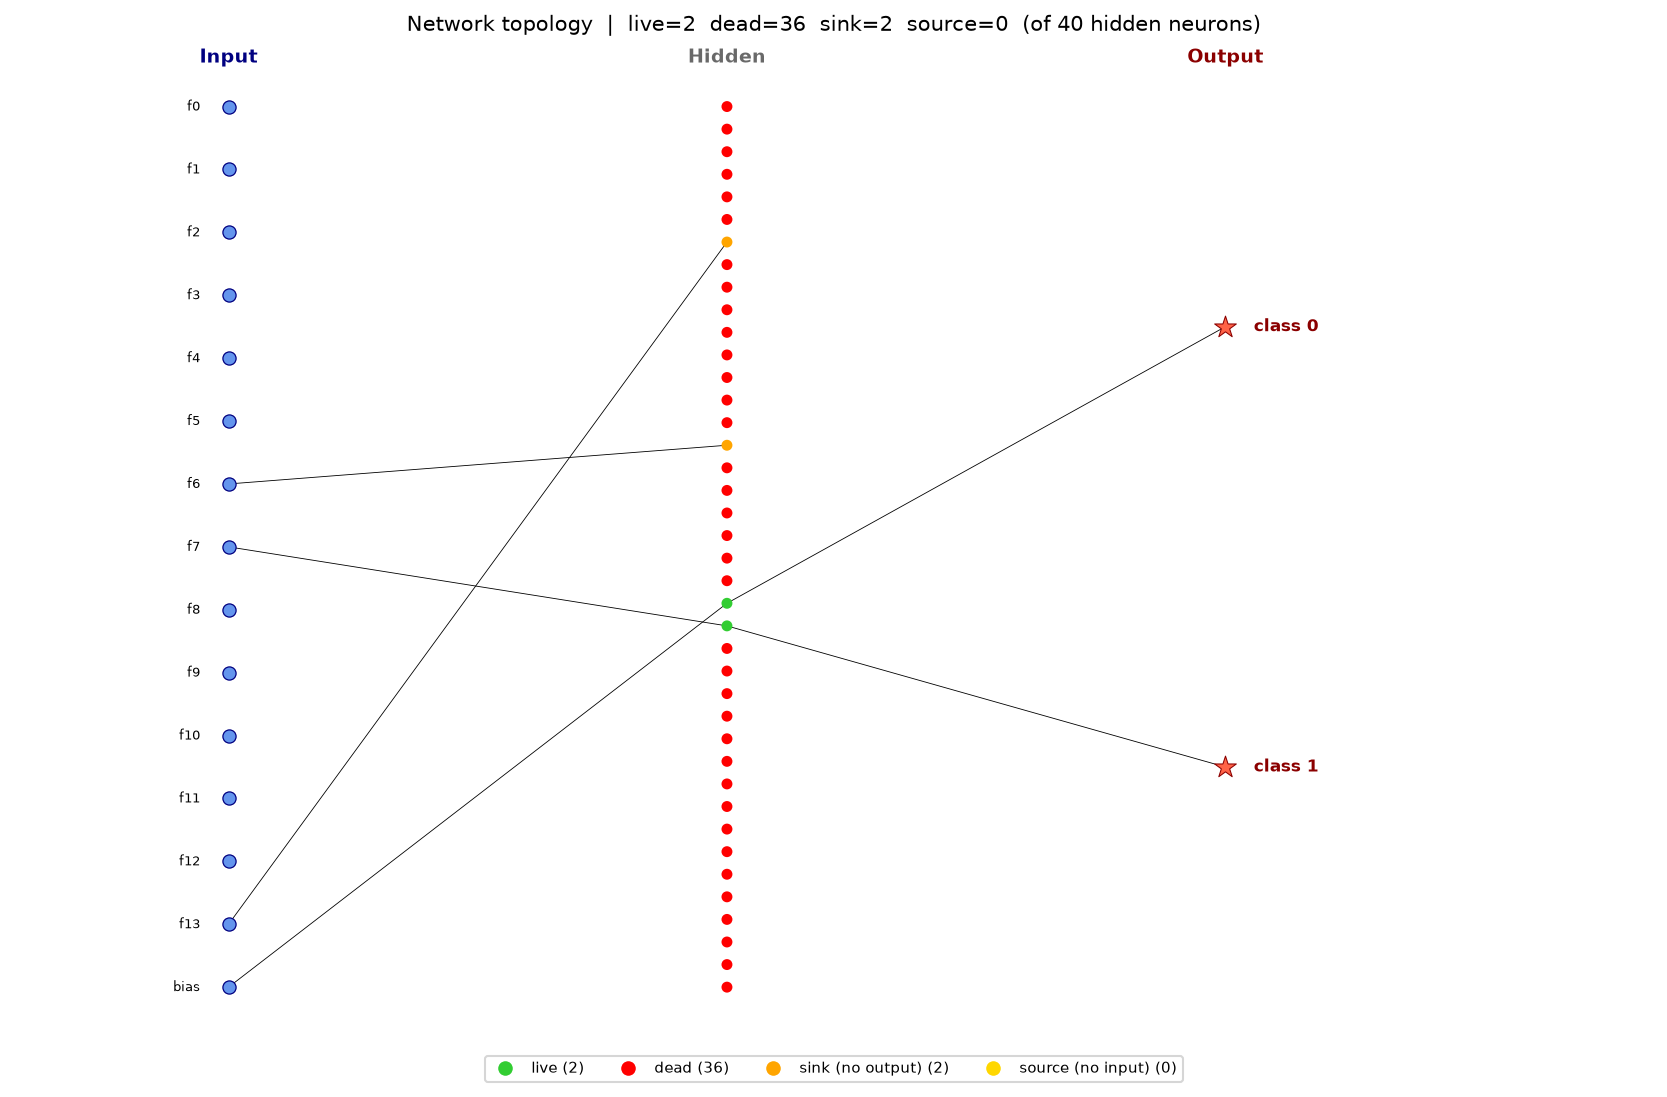
\includegraphics[height=3.1cm]{conectividad_ds1_moeackf.png}
    \end{column}
  \end{columns}
\end{frame}

% =====================================================================
\section{Cierre}
% =====================================================================
\begin{frame}{Cumplimiento de objetivos}
  \scriptsize
  \begin{tabular}{cp{10.3cm}}
    \semaforo{1} & \textbf{O1 (cumplido)}: 2 algoritmos seleccionados (MOEA-CKF, S-NSGA-II), aplicados a las 4 tareas. \\
    \semaforo{2} & \textbf{O2 (parcial)}: \textit{snn-simulator} validado estadísticamente vs.\ ANNarchy/NEST; Brian2 solo evaluado cualitativamente. \\
    \semaforo{2} & \textbf{O3 (parcial)}: migración e integración exitosas (33 tests), pero conectividad revela redes estructuralmente incoherentes. \\
    \semaforo{2} & \textbf{O4 (parcial)}: validado en 4 datasets, 31 corridas pareadas; convergencia significativa en solo 1 de 4. \\
    \semaforo{1} & \textbf{O5 (cumplido)}: comparación SNN vs.\ ANN en 8 combinaciones; salvedad de ajuste de hiperparámetros. \\
  \end{tabular}
  \vspace{4pt}
  \begin{alertblock}{Objetivo general}
    \footnotesize \textbf{Cumplido parcialmente.} Plataforma funcional y validada estadísticamente, condicionada por dos limitaciones transversales: (1) la ANN de referencia superó a la SNN en las 8 combinaciones; (2) ningún algoritmo incorpora consciencia topológica.
  \end{alertblock}
\end{frame}

% ---------------------------------------------------------------------
\begin{frame}{Trabajo futuro}
  \small
  \begin{block}{Prioritarias}
    \begin{itemize}
      \item \textbf{Operadores conscientes de topología}: inicialización/poda que garanticen un camino activo por clase y eliminen sinapsis de neuronas sumidero/fuente.
      \item \textbf{Verificar sobreajuste en el remuestreo}: medir en un conjunto de test independiente si la mejora de HV es generalización real.
      \item \textbf{Comparación SNN-ANN bajo ajuste equivalente}: repetir la búsqueda bayesiana también para la ANN.
    \end{itemize}
  \end{block}
  \footnotesize
  También: comparación empírica completa de frameworks (incluir Brian2), verificación directa de la capacidad de generalización (exactitud de test), y tratamiento del desbalance de clases en \texttt{ds2}/\texttt{ds3}.
\end{frame}

% ---------------------------------------------------------------------
\begin{frame}[plain]
  \begin{center}
    \vspace{1.2cm}
    
\includegraphics[height=1.4cm]{LogoUsachColor.png}\\[18pt]
    {\usebeamercolor[fg]{title}\Huge\bfseries ¡Gracias!}\\[10pt]
    \large Preguntas y comentarios\\[24pt]
    \small Nicolás Aguilera González\\
    \footnotesize Proyecto Fondecyt Regular 1251455 NeuroMetaEvo
  \end{center}
\end{frame}

% =====================================================================
% BACKUP
% =====================================================================
{
\setbeamercolor{frametitle}{fg=white,bg=usachgray}
\begin{frame}[plain]
  \centering
  \Large\bfseries\color{usachgray} Diapositivas de respaldo
\end{frame}

\begin{frame}{Backup --- Preguntas anticipadas}
  \small
  \textbf{P1. Si las SNN son más eficientes, ¿por qué ganó la ANN?}\\
  \footnotesize La eficiencia prometida por las SNN es \emph{energética en hardware neuromórfico}, no exactitud de clasificación en CPU/GPU convencional. Además, la ANN de referencia no fue ajustada con búsqueda bayesiana de hiperparámetros.
  \vspace{6pt}

  \small\textbf{P2. ¿Por qué no se reportó exactitud en test?}\\
  \footnotesize El estándar de la literatura de referencia (S-NSGA-II, MOEA-CKF) es reportar HV, no exactitud de test independiente. Queda identificado como trabajo futuro.
  \vspace{6pt}

  \small\textbf{P3. ¿Por qué no se trató el desbalance de clases?}\\
  \footnotesize Por fidelidad metodológica: los estudios originales de ambos algoritmos usan los mismos datasets sin tratamiento de desbalance ni discutirlo como factor de diseño.
\end{frame}

\begin{frame}{Backup --- fANOVA: los ocho estudios}
  \centering
  \begin{tabular}{ccc}
    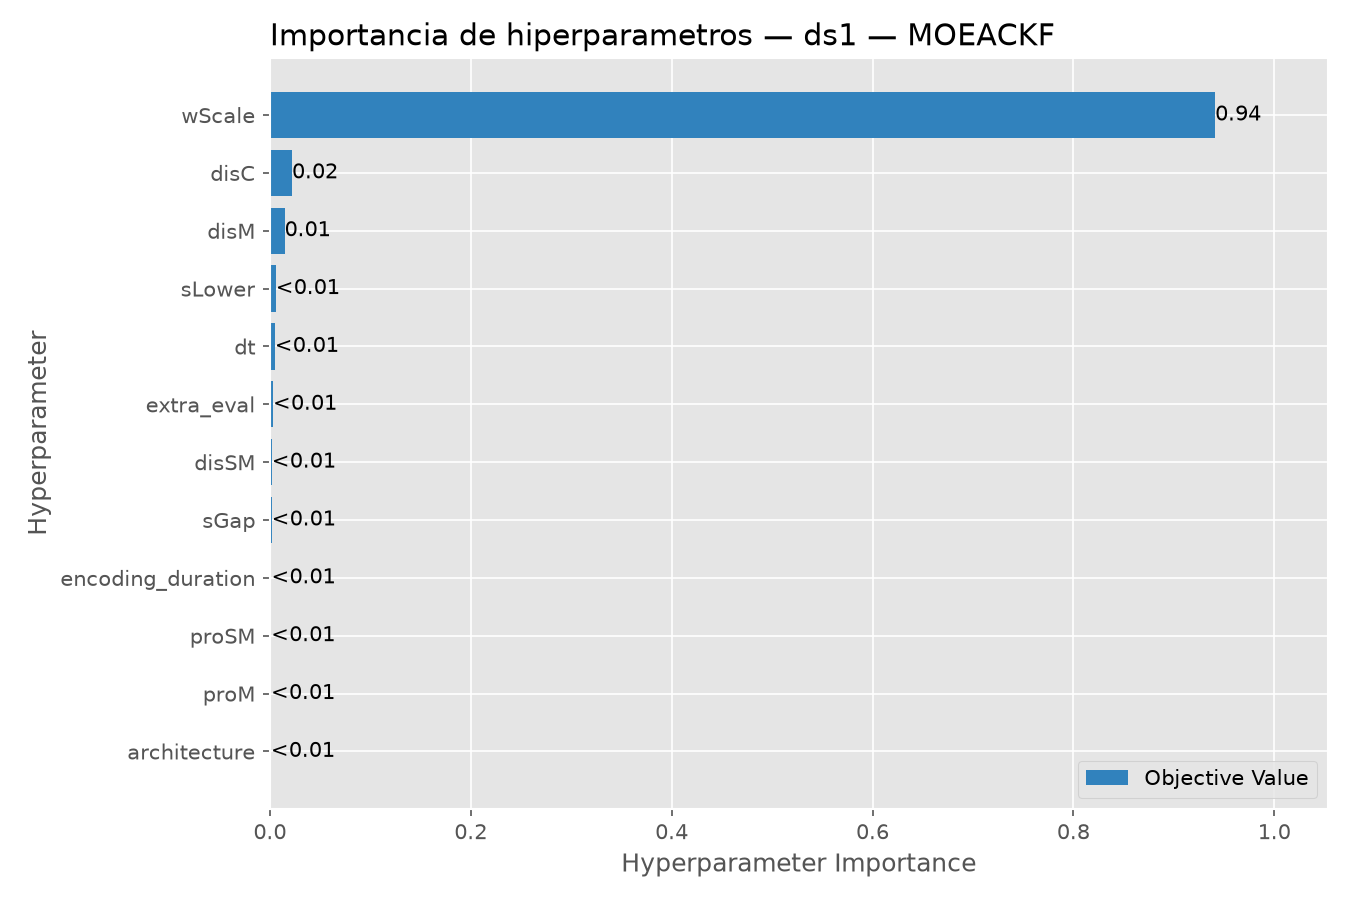
\includegraphics[width=0.3\linewidth]{importancia_MOEACKF_ds1.png} &
    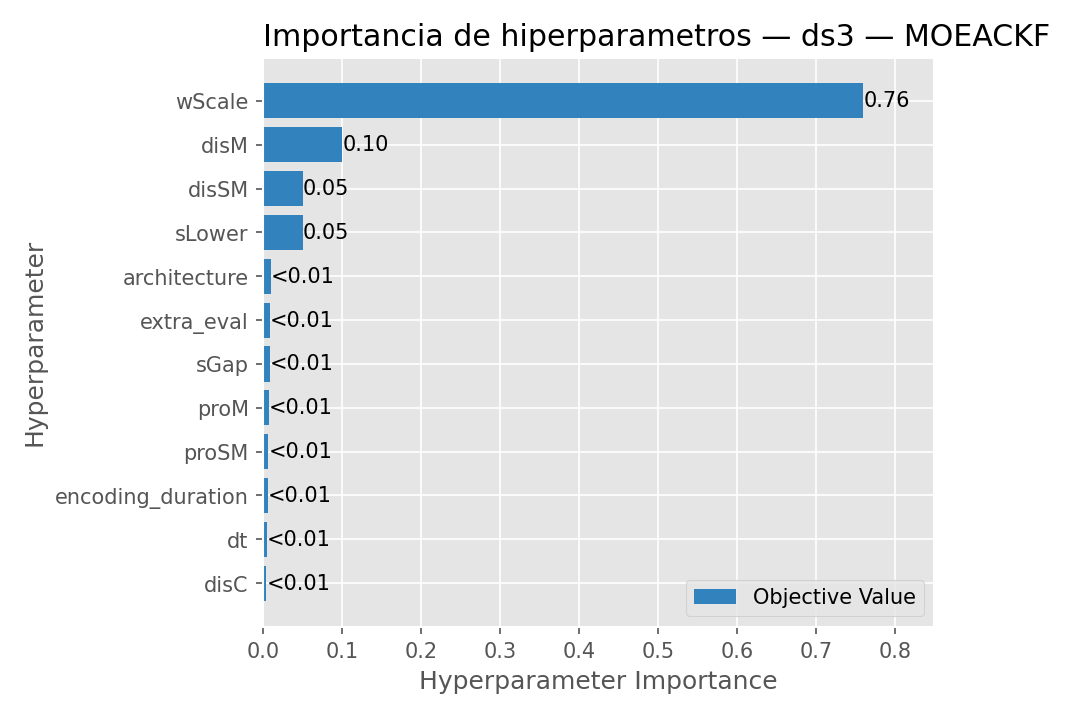
\includegraphics[width=0.3\linewidth]{importancia_MOEACKF_ds3.png} &
    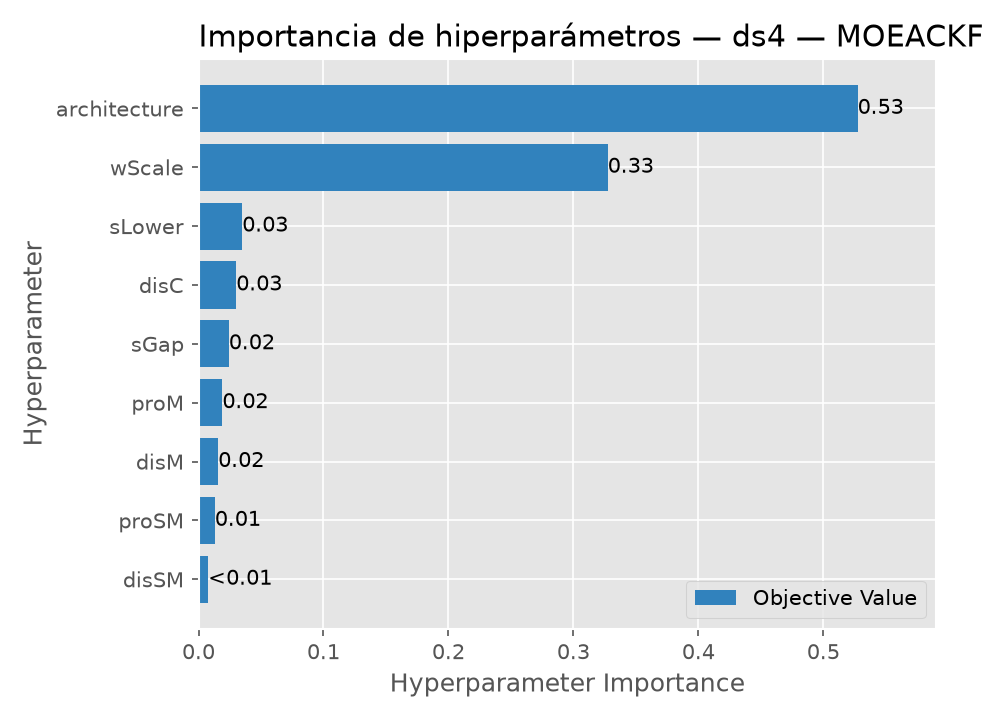
\includegraphics[width=0.3\linewidth]{importancia_MOEACKF_ds4.png} \\
    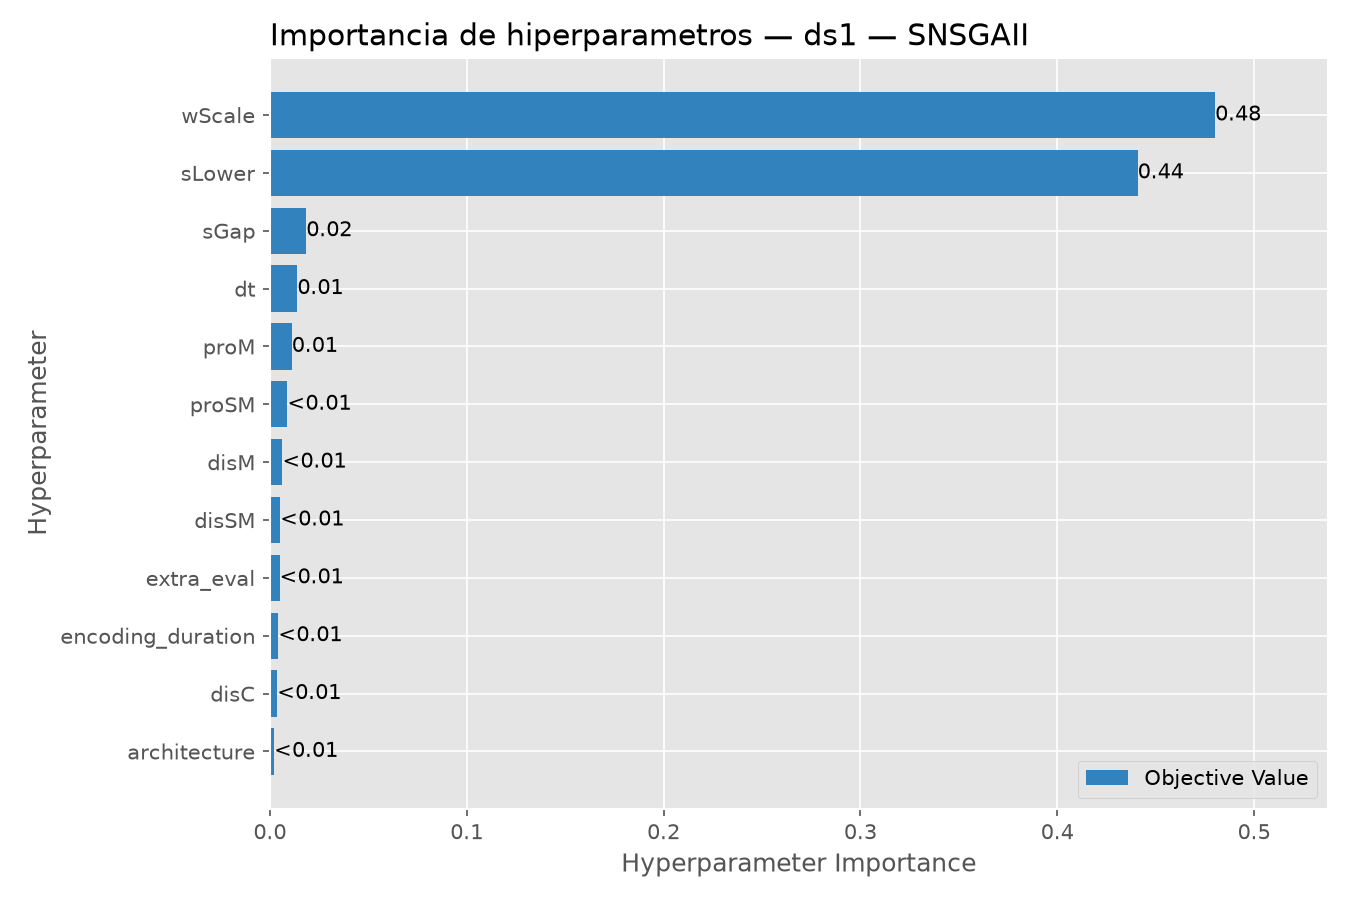
\includegraphics[width=0.3\linewidth]{importancia_SNSGAII_ds1.png} &
    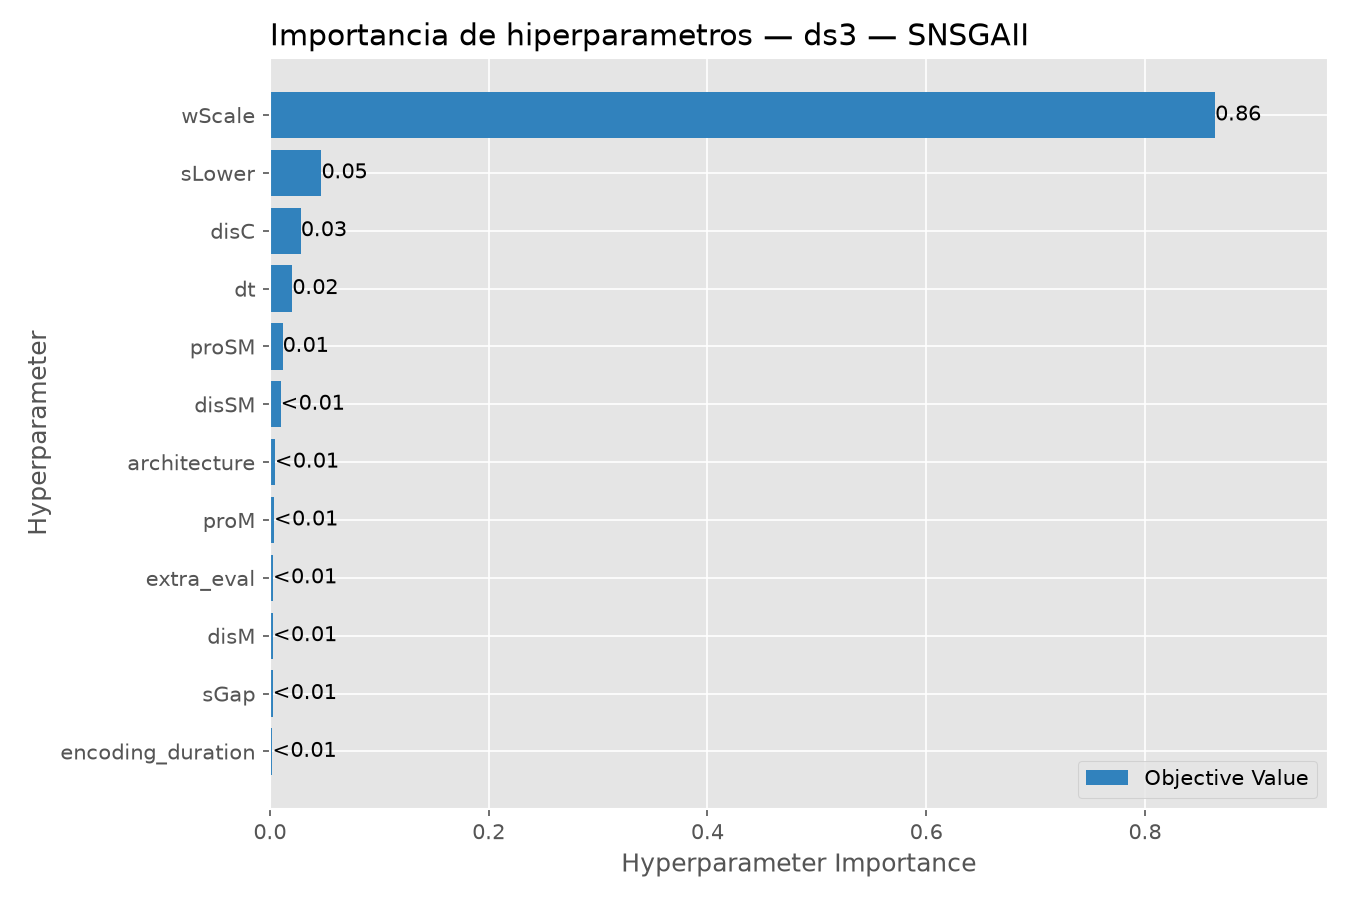
\includegraphics[width=0.3\linewidth]{importancia_SNSGAII_ds3.png} &
    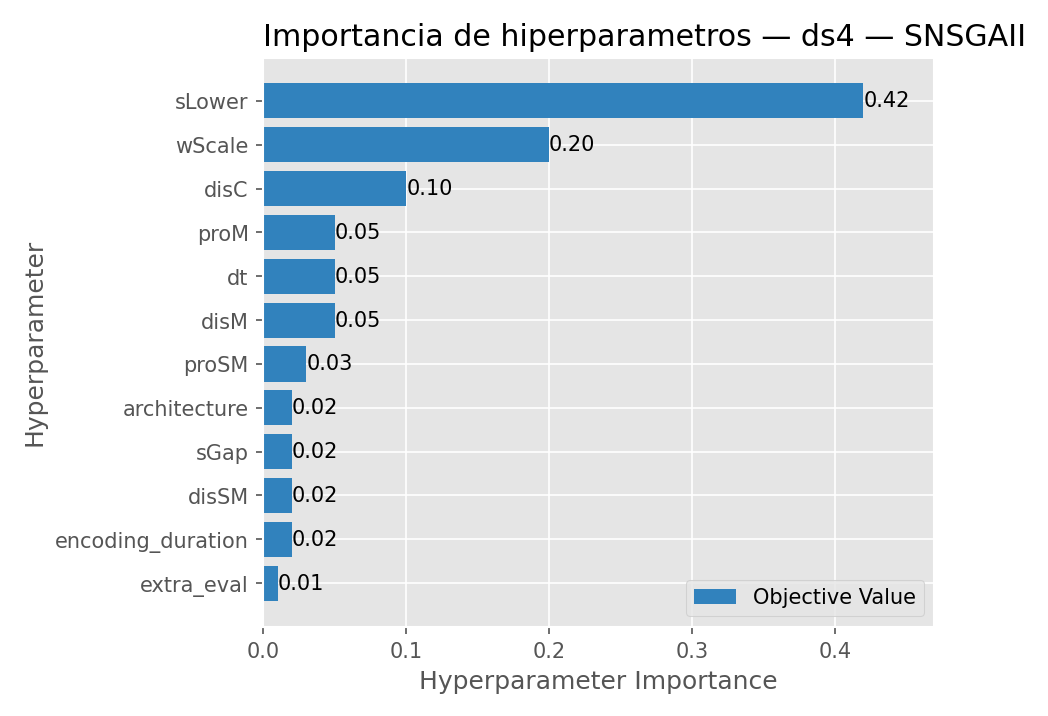
\includegraphics[width=0.3\linewidth]{importancia_SNSGAII_ds4.png}
  \end{tabular}
  \footnotesize ds2 se mostró en el bloque principal como caso representativo.
\end{frame}

\begin{frame}{Backup --- Curvas de convergencia (4 datasets)}
  \centering
  \begin{tabular}{cc}
    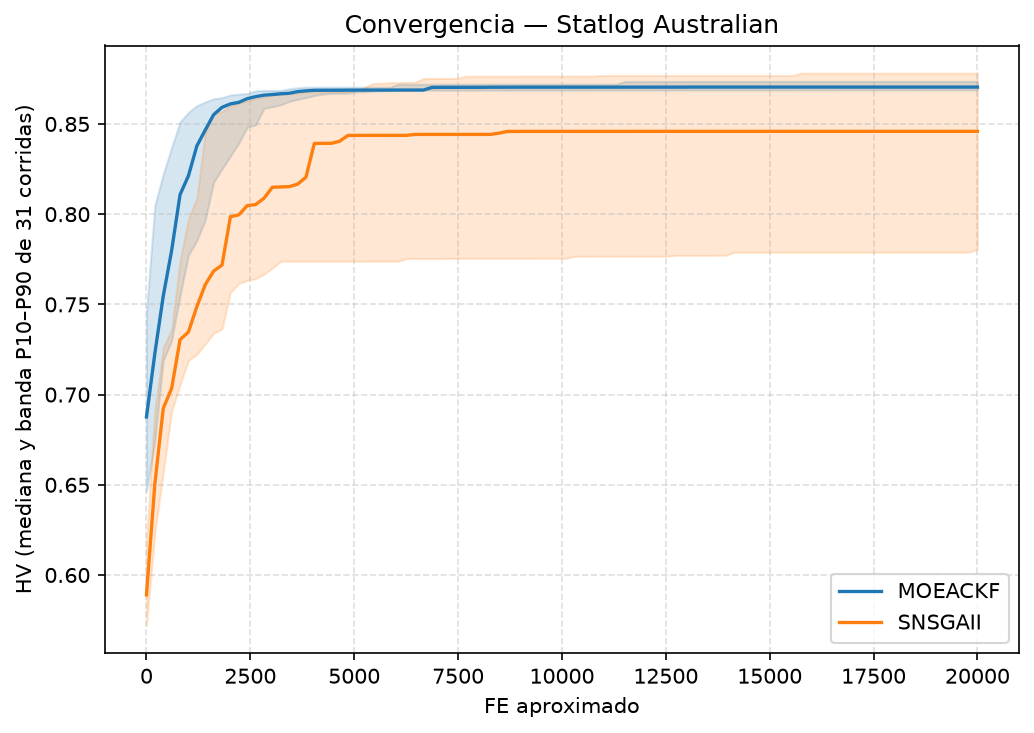
\includegraphics[height=3.1cm]{ds1_convergence.png} &
    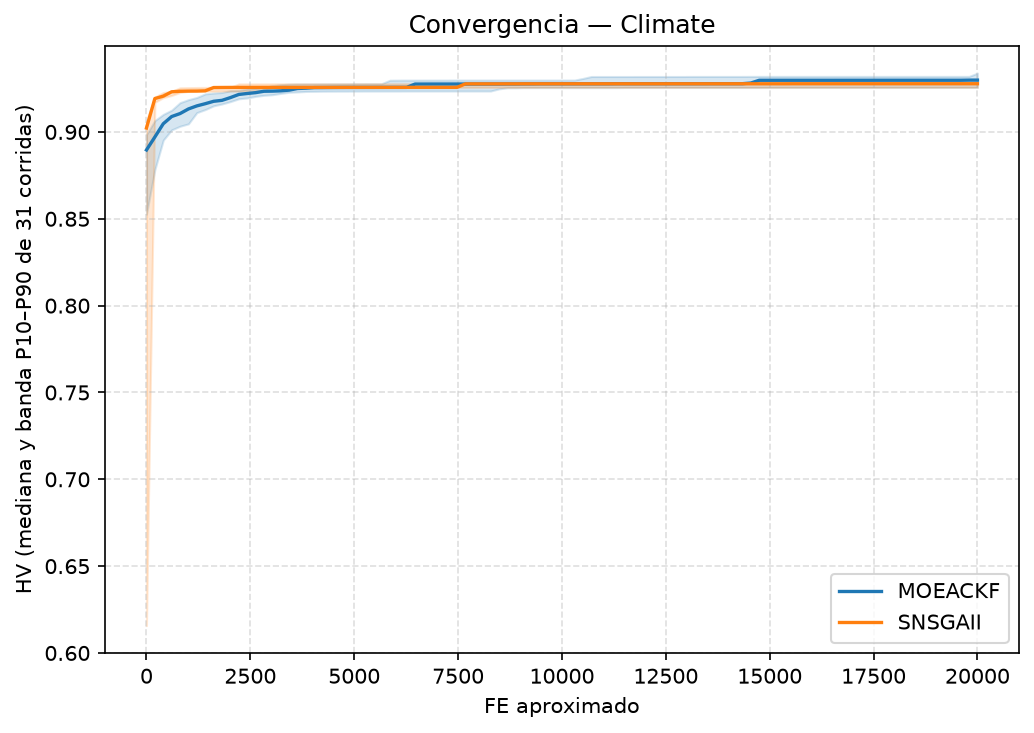
\includegraphics[height=3.1cm]{ds2_convergence.png} \\
    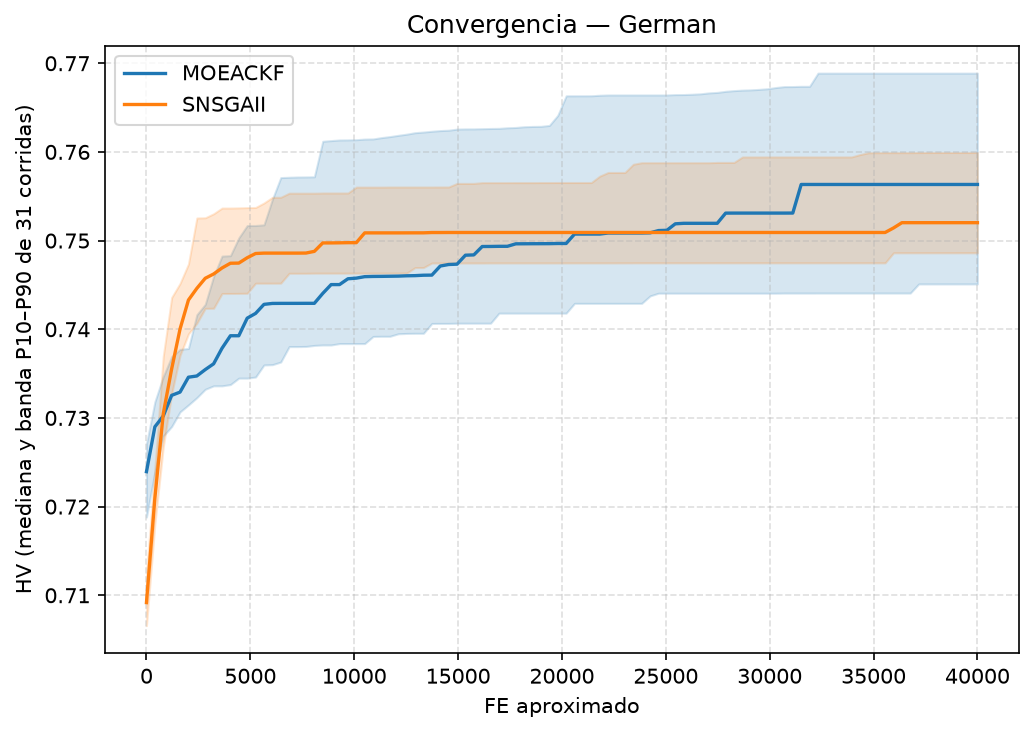
\includegraphics[height=3.1cm]{ds3_convergence.png} &
    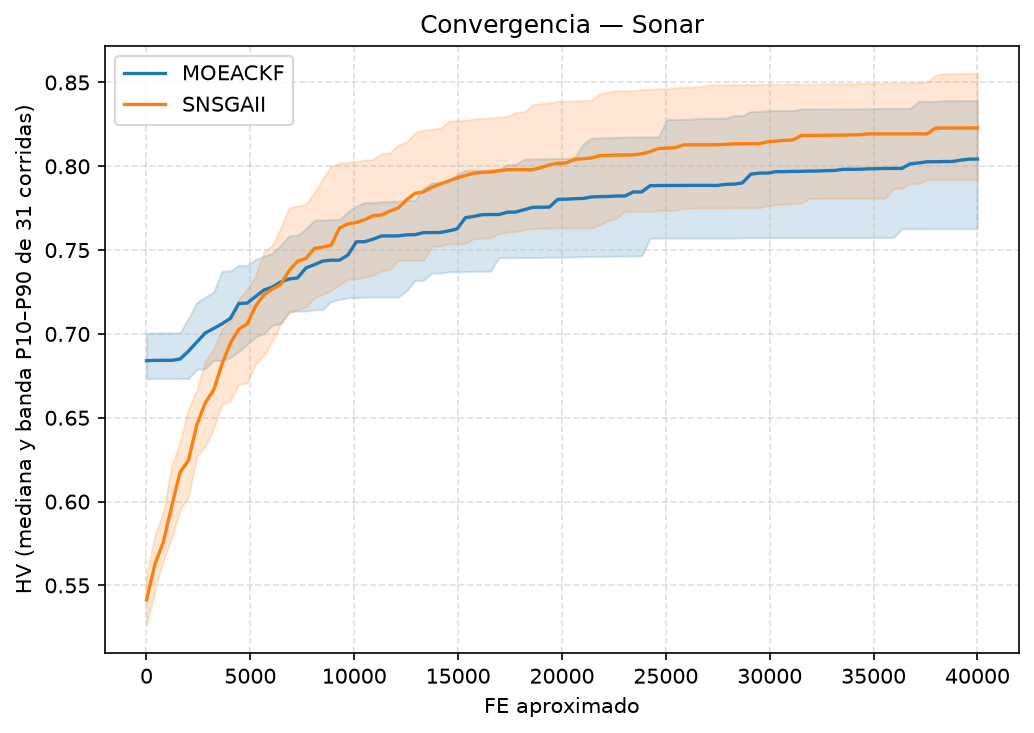
\includegraphics[height=3.1cm]{ds4_convergence.png}
  \end{tabular}
\end{frame}

\begin{frame}{Backup --- SNN vs.\ ANN, tablas completas (ds1--ds2)}
  \centering\tiny
  \begin{tabular}{lcccc}
    \toprule
    \textbf{ds1, MOEA-CKF} & SNN & ANN & $p$ & \Atwelve \\ \midrule
    HV & 0.8705 & 0.8891 & $1.37\times10^{-11}$* & 0.000 \\
    Complejidad & 0.0118 & 0.0203 & $1.99\times10^{-6}$* & 0.149 \\
    Error & 0.1413 & 0.1196 & $5.26\times10^{-12}$* & 1.000 \\ \bottomrule
  \end{tabular}
  \hspace{0.4cm}
  \begin{tabular}{lcccc}
    \toprule
    \textbf{ds1, S-NSGA-II} & SNN & ANN & $p$ & \Atwelve \\ \midrule
    HV & 0.8459 & 0.8972 & $1.54\times10^{-11}$* & 0.001 \\
    Complejidad & 0.0118 & 0.0265 & $4.88\times10^{-11}$* & 0.020 \\
    Error & 0.1685 & 0.1105 & $1.08\times10^{-11}$* & 1.000 \\ \bottomrule
  \end{tabular}

  \vspace{6pt}
  \begin{tabular}{lcccc}
    \toprule
    \textbf{ds2, MOEA-CKF} & SNN & ANN & $p$ & \Atwelve \\ \midrule
    HV & 0.9298 & 0.9767 & $1.40\times10^{-11}$* & 0.000 \\
    Complejidad & 0.0202 & 0.0487 & $1.88\times10^{-7}$* & 0.114 \\
    Error & 0.0764 & 0.0232 & $7.31\times10^{-12}$* & 1.000 \\ \bottomrule
  \end{tabular}
  \hspace{0.4cm}
  \begin{tabular}{lcccc}
    \toprule
    \textbf{ds2, S-NSGA-II} & SNN & ANN & $p$ & \Atwelve \\ \midrule
    HV & 0.9278 & 0.9477 & $1.39\times10^{-11}$* & 0.000 \\
    Complejidad & 0.0024 & 0.9114 & $5.12\times10^{-12}$* & 0.000 \\
    Error & 0.0787 & 0.0347 & $3.04\times10^{-12}$* & 1.000 \\ \bottomrule
  \end{tabular}
\end{frame}

\begin{frame}{Backup --- SNN vs.\ ANN, tablas completas (ds3--ds4)}
  \centering\tiny
  \begin{tabular}{lcccc}
    \toprule
    \textbf{ds3, MOEA-CKF} & SNN & ANN & $p$ & \Atwelve \\ \midrule
    HV & 0.7563 & 0.8098 & $1.40\times10^{-11}$* & 0.000 \\
    Complejidad & 0.0120 & 0.0413 & $1.80\times10^{-6}$* & 0.147 \\
    Error & 0.2675 & 0.2075 & $1.24\times10^{-11}$* & 1.000 \\ \bottomrule
  \end{tabular}
  \hspace{0.4cm}
  \begin{tabular}{lcccc}
    \toprule
    \textbf{ds3, S-NSGA-II} & SNN & ANN & $p$ & \Atwelve \\ \midrule
    HV & 0.7520 & 0.8119 & $1.40\times10^{-11}$* & 0.000 \\
    Complejidad & 0.0028 & 0.8751 & $1.01\times10^{-11}$* & 0.000 \\
    Error & 0.2725 & 0.2025 & $1.27\times10^{-11}$* & 1.000 \\ \bottomrule
  \end{tabular}

  \vspace{6pt}
  \begin{tabular}{lcccc}
    \toprule
    \textbf{ds4, MOEA-CKF} & SNN & ANN & $p$ & \Atwelve \\ \midrule
    HV & 0.8043 & 0.8740 & $2.06\times10^{-11}$* & 0.004 \\
    Complejidad & 0.0492 & 0.0097 & $6.61\times10^{-6}$* & 0.834 \\
    Error & 0.2096 & 0.1377 & $4.96\times10^{-11}$* & 0.985 \\ \bottomrule
  \end{tabular}
  \hspace{0.4cm}
  \begin{tabular}{lcccc}
    \toprule
    \textbf{ds4, S-NSGA-II} & SNN & ANN & $p$ & \Atwelve \\ \midrule
    HV & 0.8229 & 0.9143 & $1.70\times10^{-11}$* & 0.002 \\
    Complejidad & 0.0393 & 0.1503 & $0.0635$ (n.s.) & 0.363 \\
    Error & 0.1916 & 0.0898 & $1.30\times10^{-11}$* & 1.000 \\ \bottomrule
  \end{tabular}
\end{frame}

\begin{frame}{Backup --- Tabla A.2: fidelidad de la migración}
  \centering\scriptsize
  \begin{tabular}{p{3.6cm}p{1.6cm}p{6.2cm}}
    \toprule
    \textbf{Componente} & \textbf{Fidelidad} & \textbf{Notas} \\
    \midrule
    \texttt{vssps} (init.\ \textit{stripe}) & Alta & Lógica de franjas traducida fielmente. \\
    \texttt{ssbx} (sparse SBX) & Alta & Manejo correcto de posiciones cero/no-cero e intercambios en \textit{mismatches}. \\
    \texttt{spm} (sparse PM) & Alta & Mutación de valores y de esparsidad correctamente implementada. \\
    \texttt{sm2target} & Alta & Comportamiento fiel al original. \\
    \texttt{Environmental Selection NSGA2} & Alta & Fiel al original; corrige error de conversión \textit{inf}$\to$\textit{int}. \\
    \bottomrule
  \end{tabular}
  \vspace{4pt}
  \footnotesize Sin equivalente directo en C++/Eigen: \texttt{kmeans}, \texttt{unique(...,'rows')}, \texttt{sortrows}, \texttt{pdist2}, \texttt{randi}/\texttt{randperm}/\texttt{unifrnd} --- reimplementados con equivalencia algorítmica o exacta (detalle en Tabla A.3 de la tesis).
\end{frame}

}

\end{document}
